\documentclass[conference]{IEEEtran}
\usepackage[utf8]{inputenc}
\usepackage{graphicx}
\usepackage{booktabs}
\usepackage{adjustbox}
\usepackage{amsmath,amssymb}
\usepackage{multirow}
\usepackage{url}
\usepackage[hidelinks]{hyperref}

\title{ToonSense: Robust Multimodal Understanding of Cartoon-Driven Bangla--English Code-Mixed Memes}
\author{\IEEEauthorblockN{Adrita Biswas, Atanu Dewanjee, Hrittika Dutta}
\IEEEauthorblockA{School of Science, Engineering and Technology, East Delta University, Chattogram, Bangladesh}}

\begin{document}
\maketitle

\begin{abstract}
Multimodal meme classifiers are evaluated on clean benchmarks, yet memes circulate in Romanised spellings, with
mixed languages and degraded images. We present ToonSense, a robustness study of frozen-encoder multimodal models
for Bangla--English memes, centred on cartoon memes from CMBan and replicated on BanglaAbuseMeme and MemoSen. We
benchmark six multilingual text encoders, four image encoders and five fusion heads with repeated cross-validation
and Holm-corrected significance tests. We then subject the primary XLM-R + CLIP ViT-B/32 models to twelve
linguistic and visual perturbations at three severities, analyse attributions before and after perturbation with
Integrated Gradients and Grad-CAM, and categorise errors as linguistic, visual, cross-modal or cultural. Image
features carry most of the signal, and fusion adds a small but significant gain on the larger datasets. Romanised
Bangla is the most damaging perturbation on every dataset, reducing fusion macro-F1 by 8--21\% relative, whereas
native-script spelling noise and code-mixing are nearly harmless. The perturbed text gains rather than loses
attribution share, and visual perturbations flip up to 27\% of predictions with comparatively small F1 changes.
Training-time augmentation with transliterated copies cuts the Romanisation drop to 2--5\%, including for an unseen
spelling style, at a clean-accuracy cost below one point.
\end{abstract}

\begin{IEEEkeywords}
Bangla memes, multimodal classification, code-mixing, robustness, Romanisation, CLIP, XLM-R, explainability
\end{IEEEkeywords}
\section{Introduction}
\label{sec:intro}

Internet memes combine an image with overlaid text, and their meaning usually arises from the interaction of the
two: a harmless caption can become sarcastic or offensive in front of a particular picture, and vice versa. This
interaction makes memes hard for systems that analyse text or images in isolation. It has motivated a line of
multimodal datasets and models for sentiment, humour, offensiveness and hate
speech~\cite{kiela2020hateful,sharma2020memotion}.

Bangla is spoken by more than 250 million people, and Bangla memes have recently received dedicated
resources~\cite{hossain2022memosen,hossain2022mute,das2023banglaabusememe,hossain2024bhm}. The most recent,
CMBan~\cite{cmban2025}, focuses on \emph{cartoon-driven} memes. These are built on recurring cartoon templates and
written in Bangla, English or a mix of both, and are annotated for humour, sarcasm, offensiveness, motivation and
sentiment.

All of these works evaluate models on held-out \emph{clean} data. Social-media memes, however, are not clean.
\begin{itemize}
  \item The same joke circulates in Bangla script and in Romanised ``Banglish'', with inconsistent spelling,
  English insertions and added or stripped emojis.
  \item Images are recompressed, cropped, resized and re-captioned as they are shared.
\end{itemize}
A model that scores well on a benchmark may therefore fail on the variants it meets in deployment, for example if
it depends on surface spellings or on image details rather than on the meme's meaning. To our knowledge, no prior
work measures how Bangla meme classifiers behave under such variation.

We present \textbf{ToonSense}, a robustness study of multimodal models on Bangla--English cartoon memes. ToonSense
addresses three questions:
\begin{enumerate}
  \item[\textbf{Q1}] How much do text, image and their fusion contribute to clean-data accuracy?
  \item[\textbf{Q2}] How much does accuracy drop under realistic linguistic and visual perturbations, and which
  modality and perturbation types are most harmful?
  \item[\textbf{Q3}] Why do the models fail? Do attribution patterns shift under perturbation, and can errors be
  traced to the text, the image, their combination or cultural context?
\end{enumerate}

Our contributions are:
\begin{itemize}
  \item \textbf{A robustness framework for Bangla memes.} It covers twelve perturbation families at three
  severities. The six linguistic families include a colloquial Bangla-to-Banglish transliterator, Romanised and
  native-script spelling noise, code-mixing and emoji edits. The six visual families include text-region
  occlusion driven by OCR boxes. Performance loss is measured by the Robustness Drop and the label-free flip rate.

  \item \textbf{A multi-encoder benchmark.} We compare six frozen multilingual text encoders, four image encoders
  and five fusion heads, using repeated cross-validation, bootstrap confidence intervals and Holm-corrected
  significance tests. Besides the publicly labelled CMBan subset, we replicate all analyses on two larger Bangla
  meme datasets, BanglaAbuseMeme~\cite{das2023banglaabusememe} and MemoSen~\cite{hossain2022memosen}.

  \item \textbf{Comparative explainability.} We compare Integrated Gradients modality shares, token attributions
  and Grad-CAM maps \emph{before and after} perturbation. We introduce a text-attention ratio that measures how
  much CLIP looks at the rendered caption.

  \item \textbf{An error taxonomy} that attributes clean errors and robustness failures to linguistic, visual,
  cross-modal, OCR-related and contextual/cultural sources.
\end{itemize}

Our main findings are as follows.
\begin{itemize}
  \item Image encoders carry most of the signal: CLIP beats every frozen text encoder on all three datasets, and a
  character $n$-gram baseline beats the text encoders on the two larger ones. With a few thousand training memes,
  fusion adds a small but significant gain.
  \item Romanised Bangla is the most damaging perturbation on every dataset. It reduces the macro-F1 of the fusion
  models by 8--21\% relative and changes 26--45\% of their predictions, while native-script spelling noise and
  code-mixing are nearly harmless.
  \item Fusion halves this damage on the larger datasets but not on the small CMBan subset. On all datasets, the
  perturbed text \emph{gains} attribution share rather than being discounted.
  \item Adding transliterated copies of the training memes removes most of the drop, including for a Romanised
  spelling style never seen in training, at a cost of under one point of clean macro-F1.
  \item Visual perturbations flip up to 27\% of predictions with comparatively small F1 changes, so aggregate
  accuracy understates instability. The largest residual error class is contextual or cultural.
\end{itemize}
Code, perturbation generators and evaluation scripts are released to support reproducible robustness evaluation of
Bangla meme models.

\section{Related Work}
\label{sec:related}

\paragraph{Multimodal meme understanding.}
Memes convey meaning through the interplay of an image and overlaid text. The Hateful Memes
challenge~\cite{kiela2020hateful} showed that unimodal models fail when either modality alone is benign. Memotion
(SemEval-2020 Task~8)~\cite{sharma2020memotion} introduced the humour, sarcasm, offensiveness, motivation and
overall-sentiment taxonomy that CMBan adopts. Most systems pair a pretrained text encoder with a pretrained vision
encoder, often CLIP~\cite{radford2021clip}, and fuse the two representations.

\paragraph{Bangla meme resources.}
Bangla memes have recently received dedicated datasets.
\begin{itemize}
  \item MemoSen~\cite{hossain2022memosen} annotates 4{,}417 memes for three-way sentiment and reports that
  multimodal models outperform unimodal ones.
  \item MUTE~\cite{hossain2022mute} targets hateful memes in Bangla and code-mixed text.
  \item BHM~\cite{hossain2024bhm} adds target identification for hateful memes.
  \item BanglaAbuseMeme~\cite{das2023banglaabusememe} annotates 4{,}043 memes for abuse, vulgarity, sarcasm,
  sentiment and target.
  \item MIMOSA~\cite{ahsan2024mimosa} annotates aggression targets.
  \item CMBan~\cite{cmban2025} is the first resource built around \emph{cartoon} memes. It annotates 2{,}641
  Bangla and code-mixed memes along the five Memotion dimensions and identifies more than 800 recurring cartoon
  templates.
\end{itemize}
All of these works evaluate models on held-out \emph{clean} data. None asks whether the predictions survive the
spelling, script and image variations that memes undergo as they spread.

\paragraph{Robustness evaluation.}
Controlled corruption benchmarks such as ImageNet-C~\cite{hendrycks2019benchmarking} established severity-graded
perturbations as a standard way to measure visual robustness. In NLP, behavioural testing (CheckList;
\cite{ribeiro2020checklist}) probes models with targeted input transformations. Code-switching benchmarks such as
GLUECoS~\cite{khanuja2020gluecos} show that multilingual encoders degrade on mixed-language input. For Bangla, the
dominant real-world variation is \emph{Romanised} (``Banglish'') writing, with highly inconsistent spelling. CLIP is
known to read text rendered in images, which makes it vulnerable to typographic manipulation~\cite{goh2021multimodal}.
That property is directly relevant to memes, where the text \emph{is} part of the image.

\paragraph{Explainability for multimodal models.}
Gradient-based attribution methods such as Integrated Gradients~\cite{sundararajan2017ig} and
Grad-CAM~\cite{selvaraju2017gradcam,chattopadhay2018gradcampp} are widely used to inspect which tokens and image
regions drive a decision. Prior Bangla meme work has used explanations mainly to justify predictions. We instead use
attribution \emph{comparatively}: we measure how modality reliance and visual attention shift between the clean and
perturbed versions of the same meme.

\paragraph{Positioning.}
ToonSense is, to our knowledge, the first study of the \emph{robustness} of multimodal models on Bangla cartoon
memes. It combines a multi-encoder benchmark, Bangla-specific linguistic perturbations (colloquial transliteration,
Romanised spelling variation, code-mixing) with visual corruptions, before/after attribution analysis, and a source
attribution of errors.

% =====================================================================================
% ToonSense — Methodology section
% Required packages: graphicx, booktabs, amsmath, amssymb, multirow, (hyperref)
% Figures: figures/methodology_flow.pdf   |   Bibliography: references.bib
% Numbers in this section come from results/<dataset>/ and results/RESULTS.md (CMBan: 133-meme labelled subset,
% coarse labels; BanglaAbuseMeme and MemoSen: released labels).
% =====================================================================================

\section{Methodology}
\label{sec:method}

\subsection{Overview}
\label{sec:method:overview}

Figure~\ref{fig:flow} summarises ToonSense. The design separates the two modalities. Text is recovered from the
meme image with optical character recognition (OCR) and encoded by a frozen multilingual language model. The image
is encoded by a frozen vision encoder. A lightweight fusion head is trained on the two embeddings for each semantic
task. On top of this pipeline, linguistic and visual perturbations are injected \emph{before} the encoders, so the
same trained classifiers are evaluated on clean and perturbed versions of the same memes. The resulting predictions
feed four analyses: clean evaluation, robustness analysis, explainability, and error analysis. A fifth stage tests
whether the dominant failure can be mitigated by train-time data augmentation. The full protocol is applied to three
Bangla meme datasets.

Following the proposal, all pretrained encoders are kept frozen and their embeddings are pre-computed. This makes the
study computationally feasible and isolates the effect of a perturbation: a perturbation only changes the input to
an encoder, never the classifier that is evaluated.

\begin{figure*}[t]
  \centering
  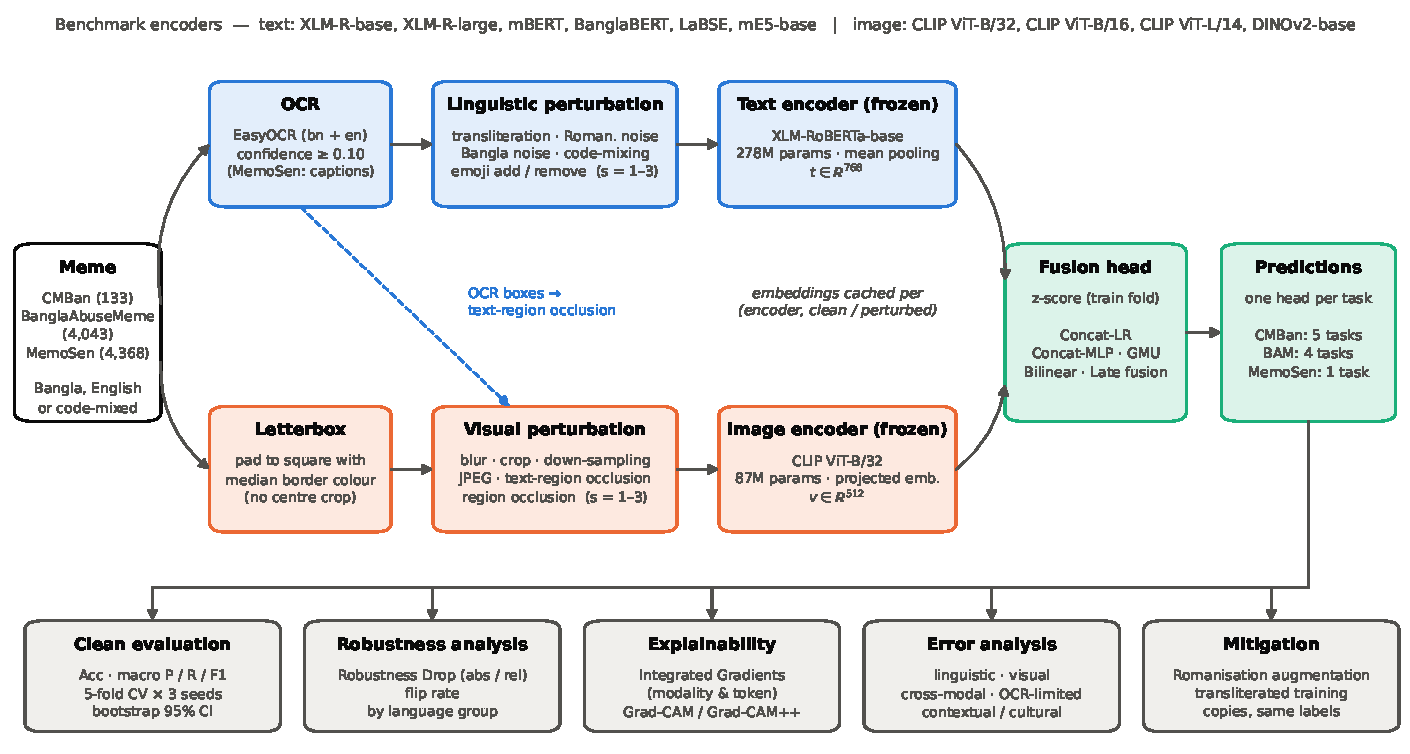
\includegraphics[width=\textwidth]{figures/methodology_flow.pdf}
  \caption{Methodology of ToonSense. Meme text is extracted with OCR (MemoSen: human-written captions) and encoded
  by XLM-RoBERTa-base; the letterboxed image is encoded by CLIP ViT-B/32. Both encoders are frozen. Controlled
  linguistic and visual perturbations (severity $s \in \{1,2,3\}$) are applied before encoding, and a separate fusion
  head is trained for each task of each dataset. OCR bounding boxes are reused to occlude rendered text. Predictions
  on clean and perturbed inputs feed the clean evaluation, robustness, explainability and error analyses, and a
  train-time Romanisation augmentation tests a mitigation. The alternative encoders listed at the top are used in the
  encoder benchmark.}
  \label{fig:flow}
\end{figure*}

% -------------------------------------------------------------------------------------
\subsection{Datasets}
\label{sec:method:data}

Table~\ref{tab:datasets} summarises the three datasets.

\paragraph{CMBan (target dataset).}
CMBan~\cite{cmban2025} contains cartoon-driven memes in Bangla, English and Bangla--English code-mixed language.
Each meme is annotated along five dimensions:
\begin{itemize}
  \item \textit{Humour}: Not Funny / Funny / Very Funny.
  \item \textit{Sarcasm}: Not / Little / Very Sarcastic.
  \item \textit{Offensiveness}: Not / Slight / Hateful Offensive.
  \item \textit{Motivation}: Not Motivational / Motivational.
  \item Overall \textit{Sentiment}: five levels from Very Negative to Very Positive.
\end{itemize}
The paper reports 2{,}641 memes, but the public release (GitHub, Hugging Face and Kaggle) provides labels for only
$N=133$; we use these. By language tag, 85 memes are Bangla, 45 code-mixed and 3 English. Several fine-grained
classes are very small (e.g.\ six \textit{Very Positive} memes). We therefore report CMBan at two granularities: the
original \emph{fine} labels, and \emph{coarse} labels that collapse intensity levels (e.g.\ Funny vs.\ Not Funny;
Negative / Neutral / Positive). Coarse labels are the primary CMBan setting. The label distribution is given in
Table~\ref{tab:data_cmban}.

\paragraph{Larger-scale Bangla meme datasets.}
To test whether our findings hold at scale, we repeat the full protocol on two public Bangla meme datasets whose
labels overlap with CMBan's tasks.
\begin{itemize}
  \item \textbf{BanglaAbuseMeme}~\cite{das2023banglaabusememe} has 4{,}043 memes annotated for sentiment
  (3 classes), sarcasm, abuse and vulgarity. Its text is rendered in the image, so it goes through the same OCR
  pipeline as CMBan.
  \item \textbf{MemoSen}~\cite{hossain2022memosen} has 4{,}368 memes with three-way sentiment and
  \emph{human-written} captions. We use the captions as the text modality, which removes OCR noise. OCR is still
  run on MemoSen to locate text regions for occlusion.
\end{itemize}
Sentiment and sarcasm correspond directly to CMBan tasks, and abuse/vulgarity are close to CMBan's offensiveness.
Neither dataset carries language tags, so we assign each meme a script group from its text: \emph{Bangla} if at
least 85\% of its letters are Bangla script, \emph{Latin-script} if at most 15\% are (English or Romanised Bangla,
which script alone cannot separate), and \emph{code-mixed} otherwise.

\begin{table*}[t]
\centering
\small
\caption{Datasets. ``Text'' is the source of the text modality; CMBan classes are given at the fine level (coarse
level in parentheses).}
\label{tab:datasets}
\begin{tabular}{lrll}
\toprule
Dataset & $N$ & Tasks (classes) & Text \\
\midrule
CMBan (released subset) & 133     & humour 3 (2), sarcasm 3 (2), offensive 3 (2), motivational 2 (2), sentiment 5 (3) & OCR \\
BanglaAbuseMeme         & 4{,}043 & sentiment (3), sarcasm (2), abuse (2), vulgarity (2)                             & OCR \\
MemoSen                 & 4{,}368 & sentiment (3)                                                                    & human \\
\bottomrule
\end{tabular}
\end{table*}

\begin{table}[t]
\centering
\small
\caption{CMBan: Label distribution of the labelled CMBan subset (N=133).}
\label{tab:data_cmban}
\begin{tabular}{lcc}
\toprule
Task & Class & n (\%) \\
\midrule
humour & Not Funny & 57 (42.9) \\
humour & Funny & 59 (44.4) \\
humour & Very Funny & 17 (12.8) \\
sarcasm & Not Sarcastic & 57 (42.9) \\
sarcasm & Little Sarcastic & 40 (30.1) \\
sarcasm & Very Sarcastic & 36 (27.1) \\
offensive & Not Offensive & 99 (74.4) \\
offensive & Slight Offensive & 20 (15.0) \\
offensive & Hateful Offensive & 14 (10.5) \\
motivational & Not Motivational & 83 (62.4) \\
motivational & Motivational & 50 (37.6) \\
sentiment & Very Negative & 11 (8.3) \\
sentiment & Negative & 25 (18.8) \\
sentiment & Neutral & 61 (45.9) \\
sentiment & Positive & 30 (22.6) \\
sentiment & Very Positive & 6 (4.5) \\
\bottomrule
\end{tabular}
\end{table}


% -------------------------------------------------------------------------------------
\subsection{Pre-processing}
\label{sec:method:prep}

\paragraph{Text extraction.}
CMBan and BanglaAbuseMeme memes carry their text \emph{inside} the image, so the text modality is obtained with
EasyOCR~\cite{easyocr} using its Bangla and English recognition models. Images whose longest side exceeds
1{,}280\,px are down-scaled before recognition. Detected fragments with confidence below $0.10$ are discarded, and
the remaining fragments are ordered top-to-bottom in line bands and left-to-right within a band.
\begin{itemize}
  \item On CMBan, OCR returns non-empty text for every meme, with a mean fragment confidence of $0.58$ and a mean
  length of 24.8 words.
  \item On BanglaAbuseMeme, the mean confidence is $0.54$ and the mean length 15.5 words.
  \item On MemoSen, the human-written captions (mean length 14.8 words) are used as text. OCR is still run, to obtain
  text boxes and OCR confidences.
\end{itemize}
The bounding box of every fragment is stored and later reused for text-region occlusion
(Section~\ref{sec:method:pert}).

\paragraph{Image normalisation.}
CLIP-style processors resize the shorter side and then centre-crop to a square. For tall multi-panel comics, which
are common in CMBan, this removes the first and last panels. We therefore \emph{letterbox} each image to a square,
padding with its median border colour, before the encoder's standard $224\times224$ preprocessing. The encoder thus
sees the complete meme.

% -------------------------------------------------------------------------------------
\subsection{Encoders}
\label{sec:method:enc}

\paragraph{Primary configuration.}
The primary model pairs \textbf{XLM-RoBERTa-base} (XLM-R)~\cite{conneau2020xlmr} as the text encoder with
\textbf{CLIP ViT-B/32}~\cite{radford2021clip} as the image encoder. For XLM-R, a text is tokenised (at most 256
tokens) and mean-pooled over the final hidden states, giving $\mathbf{t}\in\mathbb{R}^{768}$. For CLIP, we use the
projected image embedding of the vision tower, $\mathbf{v}\in\mathbb{R}^{512}$. Both encoders are frozen.

\paragraph{Benchmark encoders.}
To situate this choice, we benchmark six text and four image encoders (Table~\ref{tab:encoders}).
\begin{itemize}
  \item Text, multilingual: XLM-R-large~\cite{conneau2020xlmr} and mBERT~\cite{devlin2019bert}.
  \item Text, Bangla-specific: BanglaBERT~\cite{bhattacharjee2022banglabert}.
  \item Text, sentence-embedding models: LaBSE~\cite{feng2022labse} and multilingual-E5-base~\cite{wang2024me5}.
  \item Image, language-supervised: CLIP ViT-B/16 and ViT-L/14~\cite{radford2021clip}.
  \item Image, self-supervised (no language supervision): DINOv2-base~\cite{oquab2024dinov2}.
\end{itemize}

\begin{table}[t]
\centering
\small
\caption{Frozen encoders. Parameter counts are for the encoder actually used (for CLIP, the vision tower only).
$^\star$ marks the primary configuration.}
\label{tab:encoders}
\begin{adjustbox}{max width=\columnwidth}
\begin{tabular}{llrrl}
\toprule
Modality & Encoder & Params & Dim. & Pooling \\
\midrule
\multirow{6}{*}{Text}
 & XLM-R-base$^\star$ & 278M & 768  & mean \\
 & XLM-R-large        & 560M & 1024 & mean \\
 & mBERT (cased)      & 178M & 768  & mean \\
 & BanglaBERT         & 110M & 768  & mean \\
 & LaBSE              & 471M & 768  & pooler, $\ell_2$ \\
 & mE5-base           & 278M & 768  & mean, $\ell_2$ \\
\midrule
\multirow{4}{*}{Image}
 & CLIP ViT-B/32$^\star$ & 87M  & 512  & projection \\
 & CLIP ViT-B/16         & 86M  & 512  & projection \\
 & CLIP ViT-L/14         & 303M & 768  & projection \\
 & DINOv2-base           & 87M  & 1536 & [CLS; mean patch] \\
\bottomrule
\end{tabular}
\end{adjustbox}
\end{table}

% -------------------------------------------------------------------------------------
\subsection{Fusion and Classification Heads}
\label{sec:method:heads}

Embeddings are z-score standardised with statistics from the training fold only. A separate head is trained for each
task. Let $\mathbf{t}$ and $\mathbf{v}$ be the standardised text and image embeddings, $H=256$ the hidden size, and
$C$ the number of classes.

\paragraph{Unimodal heads.}
(i) An $\ell_2$-regularised logistic regression (LR). (ii) A two-layer MLP:
$\mathrm{Dropout}\!\to\!\mathrm{Linear}(d,H)\!\to\!\mathrm{GELU}\!\to\!\mathrm{Dropout}\!\to\!\mathrm{Linear}(H,C)$.

\paragraph{Early fusion.}
The LR or MLP above applied to the concatenation $[\mathbf{t};\mathbf{v}]$ (\emph{Concat-LR}, \emph{Concat-MLP}).

\paragraph{Gated Multimodal Unit (GMU).}
Following~\cite{arevalo2017gmu}, a learned gate decides, per hidden unit, how much each modality contributes:
\begin{equation}
\begin{aligned}
\mathbf{h}_t&=\tanh(W_t\mathbf{t}),\quad \mathbf{h}_v=\tanh(W_v\mathbf{v}),\quad \mathbf{z}=\sigma\!\left(W_z[\mathbf{t};\mathbf{v}]\right),\\
\mathbf{h}&=\mathbf{z}\odot\mathbf{h}_t+(1-\mathbf{z})\odot\mathbf{h}_v ,
\end{aligned}
\end{equation}
followed by a linear classifier on $\mathbf{h}$. The mean gate value is logged as a measure of reliance on text.

\paragraph{Bilinear interaction.}
Both modalities are projected to a shared space, $\mathbf{a}=\tanh(P_t\mathbf{t})$ and
$\mathbf{b}=\tanh(P_v\mathbf{v})$, and an MLP classifies
$[\mathbf{a};\,\mathbf{b};\,\mathbf{a}\odot\mathbf{b};\,|\mathbf{a}-\mathbf{b}|]$. This captures multiplicative
cross-modal interactions.

\paragraph{Late fusion.}
The class probabilities of the text-MLP and image-MLP are averaged:
$\hat{p}=\tfrac12\big(p_{\text{text}}+p_{\text{image}}\big)$.

\paragraph{Baselines.}
A majority-class predictor, and a character $n$-gram ($n=2$--$5$) TF-IDF + LR classifier on the OCR text. The latter
is script-agnostic and therefore a strong lexical baseline for code-mixed input.

\paragraph{Training.}
Neural heads are trained full-batch with AdamW (learning rate $10^{-3}$, weight decay $10^{-2}$), dropout $0.3$ and
class-weighted cross-entropy, for at most 300 epochs. Early stopping (patience 30) is based on the loss on an inner
validation split, and the best checkpoint is restored. For the LR heads, the inverse regularisation strength
$C\in\{0.01,0.1,1\}$ is selected on the same validation split, with balanced class weights.

% -------------------------------------------------------------------------------------
\subsection{Rationale for XLM-R + CLIP ViT-B/32}
\label{sec:method:why}

We adopt XLM-R-base + CLIP ViT-B/32 as the primary configuration for the reasons below. We stress that the choice
rests on the \emph{accuracy--efficiency trade-off} and on suitability for the data, \emph{not} on this pair
achieving the highest clean score in our benchmark.

\begin{enumerate}
  \item \textbf{Coverage of Bangla and code-mixing.} XLM-R is pretrained on CommonCrawl text in 100 languages,
  Bengali included~\cite{conneau2020xlmr}. Its SentencePiece vocabulary represents Bangla script, English and
  Romanised Bangla within a single model. This matters for CMBan, where 34\% of the labelled memes are code-mixed.
  A Bangla-only model such as BanglaBERT is not designed for English or Romanised tokens.

  \item \textbf{Language-supervised visual features.} CLIP is trained contrastively on image--text
  pairs~\cite{radford2021clip}. Its embedding therefore encodes the high-level semantics (scenes, characters,
  expressions) that meme interpretation depends on, rather than low-level appearance alone.

  \item \textbf{Competitive accuracy.} Among the 51 fusion configurations of the benchmark, the best primary head is
  1.7 (CMBan), 1.9 (BanglaAbuseMeme) and 2.6 (MemoSen) macro-F1 points behind the top configuration
  (Table~\ref{tab:cross_bench}). On CMBan the gap is not significant after Holm correction. Almost all of the gap is
  due to the image encoder: every top configuration uses CLIP ViT-L/14, which is 2.7--2.8 points better than
  ViT-B/32 as a unimodal model on all three datasets. The text encoder matters much less. With CLIP ViT-B/32 as the
  image encoder, XLM-R-base is the best text partner on CMBan (49.6\% vs.\ $\leq$48.3\%; best head per task) and
  within 0.2 points of the best on BanglaAbuseMeme and MemoSen.

  \item \textbf{Efficiency.} CLIP ViT-B/32 is the smallest image encoder considered (87M parameters). It encodes
  the 133 memes in about 15\,s on a CPU, compared with about 150\,s for ViT-L/14 (303M). XLM-R-large doubles the
  parameter count of XLM-R-base (560M vs.\ 278M) yet improves the text-only task-averaged macro-F1 by only 0.1--2.4
  points across the three datasets. The robustness protocol re-encodes 36 perturbed variants of the data, so encoder
  cost multiplies. The smaller pair keeps the CMBan study runnable on a CPU and the full study on the larger
  datasets within a single free GPU session (about 4--6\,h on a Tesla T4 per dataset).

  \item \textbf{Comparability.} XLM-R and CLIP are among the most widely used encoders in multimodal meme research,
  which makes our robustness findings comparable with prior work. The full benchmark
  (Section~\ref{sec:results:benchmark}) reports every alternative, so readers can judge the trade-off themselves.
\end{enumerate}

% -------------------------------------------------------------------------------------
\subsection{Controlled Perturbations}
\label{sec:method:pert}

We design six linguistic and six visual perturbation families, each at three severities
(Table~\ref{tab:perturbations}), mirroring how memes are altered as they circulate on social media. Every
perturbation is deterministic given the meme identifier, family and severity (a CRC32-seeded generator), so all
models see identical perturbed inputs. For linguistic perturbations, we record the token-level edit rate
(one minus the \texttt{difflib} similarity ratio over whitespace tokens) to report how much of each text actually
changed.

\paragraph{Linguistic.}
\begin{itemize}
  \item \emph{Transliteration} uses a rule-based Bangla$\to$Romanised-Bangla converter written for this study. It
  follows colloquial social-media conventions rather than a formal scheme: inherent-vowel insertion, schwa deletion
  word-finally and in VC\_CV contexts, \textit{ya-}/\textit{ba-phala}, and nukta forms.
  \item \emph{Romanised spelling noise} first romanises the text fully, then applies common Banglish spelling
  variants (e.g.\ \textit{sh}$\leftrightarrow$\textit{s}, \textit{bh}$\to$\textit{v}, \textit{i}$\to$\textit{ee},
  vowel dropping, character repetition, adjacent swaps).
  \item \emph{Bangla spelling noise} substitutes orthographically confusable characters (short/long vowel signs,
  the three sibilants, dental/retroflex nasals, etc.) or drops a vowel sign.
  \item \emph{Code-mixing} switches words between Bangla and English using a bilingual lexicon of about 200
  frequent meme words, with Bangla suffix stripping.
  \item \emph{Emoji insertion} inserts emojis from a mixed-sentiment pool.
  \item \emph{Emoji removal} strips emojis, then emoticons, then all symbols.
\end{itemize}

\paragraph{Visual.}
\begin{itemize}
  \item Blur strength is defined at the encoder's $224$-px scale, so it is independent of image resolution.
  \item \emph{Text-region occlusion} fills OCR text boxes with their median colour, removing the rendered text
  while adding minimal artefacts.
  \item \emph{Region occlusion} greys out cells of a $12\times12$ grid, restricted to cells that overlap OCR text
  by less than 20\%. It removes pictorial evidence while leaving the text intact.
\end{itemize}

\begin{table}[t]
\centering
\small
\caption{Perturbation families and severities ($s=1/2/3$).}
\label{tab:perturbations}
\begin{adjustbox}{max width=\columnwidth}
\begin{tabular}{lll}
\toprule
 & Family & Parameter at $s=1/2/3$ \\
\midrule
\multirow{6}{*}{\rotatebox{90}{Linguistic}}
 & Transliteration          & 33 / 66 / 100\% of Bangla words romanised \\
 & Romanised spelling noise & 15 / 30 / 50\% of words varied (after full romanisation) \\
 & Bangla spelling noise    & 10 / 20 / 35\% of Bangla words misspelt \\
 & Code-mixing              & switch probability 0.33 / 0.66 / 1.0 \\
 & Emoji insertion          & 1 / 3 / 6 emojis \\
 & Emoji removal            & emojis / + emoticons / + all symbols \\
\midrule
\multirow{6}{*}{\rotatebox{90}{Visual}}
 & Gaussian blur     & $\sigma$ = 1 / 2 / 4 (224-px scale) \\
 & Random crop       & 85 / 70 / 55\% of area kept \\
 & Down-sampling     & longest side 160 / 96 / 48\,px, then up-sampled \\
 & JPEG compression  & quality 30 / 15 / 5 \\
 & Text-region occl. & 33 / 66 / 100\% of OCR boxes filled \\
 & Region occlusion  & 10 / 25 / 40\% of non-text area greyed \\
\bottomrule
\end{tabular}
\end{adjustbox}
\end{table}

In the main (\emph{decoupled}) setting, a linguistic perturbation changes only the text input and a visual
perturbation changes only the image input. This attributes each effect to a single modality. A \emph{coupled}
variant, in which the text of a visually perturbed meme is re-extracted by OCR, is supported by the framework and
models deployment conditions.

% -------------------------------------------------------------------------------------
\subsection{Evaluation Protocol}
\label{sec:method:eval}

\paragraph{Cross-validation.}
On the labelled CMBan subset, a single held-out test split would contain about 27 memes and give unstable estimates.
We therefore use stratified 5-fold cross-validation, repeated with three random seeds, and apply the same protocol
to BanglaAbuseMeme and MemoSen so that all results are directly comparable.
\begin{itemize}
  \item In each fold, 80\% of the memes are used for training and 20\% for testing.
  \item A stratified 15\% of the training portion is held out as the validation split for early stopping and
  hyperparameter selection, so test folds are never used for model selection.
  \item Each meme receives exactly one out-of-fold (OOF) prediction per seed, and all metrics are computed on the
  full set of OOF predictions.
\end{itemize}

\paragraph{Metrics.}
We report accuracy and macro-averaged precision, recall and F1, as mean $\pm$ standard deviation over seeds. Macro-F1
is the primary metric because of class imbalance:
\begin{equation}
\text{Macro-F1}=\frac{1}{C}\sum_{c=1}^{C}\frac{2\,P_c R_c}{P_c+R_c}.
\end{equation}
We compute 95\% confidence intervals by bootstrap resampling (1{,}000 resamples) of the seed-ensembled predictions.
The best fusion model is compared with the best text-only and best image-only models using a paired bootstrap test,
with Holm correction across the tasks of each dataset~\cite{holm1979}. For CMBan, each task is reported at its
primary (coarse) level; the fine level is reported in the appendix.

\paragraph{Robustness.}
Each fold's model is trained once on clean data and then applied to the clean and perturbed versions of its own test
fold. For a model $f$, data $\mathcal{D}$ and perturbation $\pi_s$ at severity $s$, the \emph{Robustness Drop} is
\begin{equation}
\begin{aligned}
\mathrm{RD}_{\text{abs}}&=\mathrm{F1}(f;\mathcal{D})-\mathrm{F1}\big(f;\pi_s(\mathcal{D})\big),\\
\mathrm{RD}_{\text{rel}}&=100\cdot\frac{\mathrm{RD}_{\text{abs}}}{\mathrm{F1}(f;\mathcal{D})}.
\end{aligned}
\end{equation}
Because macro-F1 is noisy on small test sets, we also report the label-free \emph{flip rate}: the fraction of memes
whose prediction changes under the perturbation,
$\mathrm{FR}=\frac{1}{N}\sum_{i}\mathbf{1}\big[f(x_i)\neq f(\pi_s(x_i))\big]$.
All robustness measures are additionally broken down by language group: Bangla, code-mixed and (on BanglaAbuseMeme
and MemoSen) Latin-script memes. Robustness is evaluated for the primary encoder pair and all of its heads, over
$12$ families $\times$ $3$ severities $=36$ perturbed copies of every test fold.

% -------------------------------------------------------------------------------------
\subsection{Mitigation: Romanisation Augmentation}
\label{sec:method:aug}

Romanisation turns out to be the most damaging perturbation (Section~\ref{sec:results:rob}). We therefore test
whether it can be mitigated by train-time data augmentation, without collecting new labels. Let $\mathcal{T}$ be the
training portion of a fold and $\mathcal{V}\subset\mathcal{T}$ its inner validation split. The augmented training
set adds a copy of every non-validation training meme in which only the text is replaced by its perturbed version,
\begin{equation}
\mathcal{T}_{\text{aug}}=\mathcal{T}\;\cup\;\big\{\big(\pi_{s}(t_i),\,\mathbf{v}_i,\,y_i\big)
\;:\; i\in\mathcal{T}\setminus\mathcal{V},\ \pi_s\in\Pi\big\},
\end{equation}
where $\mathbf{v}_i$ is the clean image embedding and $y_i$ the original label. Copies are never made of validation
or test memes, so model selection and evaluation are not contaminated. We compare three settings:
\begin{itemize}
  \item \emph{none}: clean training data, identical to the robustness analysis.
  \item \emph{+translit.}: $\Pi=\{$transliteration, $s=2\}$. Romanised spelling noise is \emph{not} seen during
  training, so performance under it measures generalisation to an unseen Romanisation style.
  \item \emph{+translit.\ + noise}: $\Pi=\{$transliteration, $s=2$; Romanised spelling noise, $s=2\}$, an upper
  bound in which the test-time noise style is also seen during training.
\end{itemize}
All other components (primary encoder pair, text-only and fusion heads, folds and seeds) are those of the
robustness analysis, so differences are attributable to the augmentation alone. Each setting is evaluated on the
clean test folds and on all linguistic perturbations at all severities. The Robustness Drop is computed relative to
the clean macro-F1 of the same setting, so that any change in clean accuracy is reported separately.

% -------------------------------------------------------------------------------------
\subsection{Explainability}
\label{sec:method:xai}

\paragraph{Modality reliance.}
We apply Integrated Gradients (IG)~\cite{sundararajan2017ig} to the input $\mathbf{x}=[\mathbf{t};\mathbf{v}]$ of the
fusion head, using the training mean as baseline $\mathbf{x}'$ and $m=32$ midpoint Riemann steps:
\begin{equation}
\mathrm{IG}_j(\mathbf{x})=(x_j-x'_j)\int_{0}^{1}
\frac{\partial F_{\hat{y}}\big(\mathbf{x}'+\alpha(\mathbf{x}-\mathbf{x}')\big)}{\partial x_j}\,d\alpha ,
\end{equation}
where $F_{\hat{y}}$ is the logit of the predicted class. The \emph{text share} of a decision is
$\|\mathrm{IG}_{\mathbf{t}}\|_1/(\|\mathrm{IG}_{\mathbf{t}}\|_1+\|\mathrm{IG}_{\mathbf{v}}\|_1)$. It is computed
for every meme on clean and perturbed inputs to measure how perturbations shift reliance between modalities.

\paragraph{Token attribution.}
For memes whose correct prediction flips under a linguistic perturbation, IG is propagated through XLM-R to the input
token embeddings, using a pad-token baseline that keeps special tokens fixed. Sub-word attributions are summed into
words, and the clean and perturbed texts are compared.

\paragraph{Visual attribution.}
We apply Grad-CAM~\cite{selvaraju2017gradcam} and Grad-CAM++~\cite{chattopadhay2018gradcampp} to CLIP ViT-B/32 by
treating the patch tokens as a spatial feature map. The hook is placed at the \emph{input} of the last transformer
block: at its output, only the class token reaches the projection, so patch gradients would vanish. With
activations $A\in\mathbb{R}^{P\times D}$ and target logit $y^{c}$,
\begin{equation}
w_k=\frac{1}{P}\sum_{p}\frac{\partial y^{c}}{\partial A_{p,k}},\qquad
L^{c}_{p}=\mathrm{ReLU}\Big(\sum_k w_k A_{p,k}\Big).
\end{equation}
From the map we derive two quantities:
\begin{itemize}
  \item The \emph{text-attention ratio}: the share of CAM mass inside OCR text boxes divided by the boxes' share of
  the image area. A value above 1 means the model over-attends to rendered text.
  \item \emph{CAM stability}: the Pearson correlation between clean and perturbed maps, computed for the spatially
  aligned perturbations (blur, JPEG, down-sampling and both occlusions) at severity 2.
\end{itemize}
IG modality shares are computed for every meme. Grad-CAM requires a backward pass through CLIP per meme and
perturbation, so on the two larger datasets it is computed on a stratified subsample of at most 300 memes per task.

% -------------------------------------------------------------------------------------
\subsection{Error Analysis}
\label{sec:method:errors}

Errors of the primary fusion model (the best \emph{learned} XLM-R + CLIP-B/32 fusion head per task) are attributed
to a source by comparing its seed-ensembled out-of-fold predictions with those of the text-MLP and image-MLP trained
on the same folds. Late fusion is excluded here: it averages the two unimodal models, so for binary tasks it cannot
be wrong when both are right, and the cross-modal category would be empty by construction. The categories are:
\begin{itemize}
  \item \emph{linguistic}: the text model is wrong and the image model right.
  \item \emph{visual}: the image model is wrong and the text model right.
  \item \emph{cross-modal}: both unimodal models are right but fusion is wrong.
  \item \emph{OCR-limited}: all three models are wrong and the OCR text is empty or has confidence below 0.5.
  \item \emph{contextual/cultural}: all three models are wrong although usable text is available.
\end{itemize}
The contextual/cultural category is treated as a set of \emph{candidates}, which annotators verify for cultural
references.

Robustness failures are categorised analogously. A meme is \emph{linguistic-}, \emph{visual-} or
\emph{cross-modal-fragile} if its correct clean prediction becomes wrong at severity $\geq2$ under a linguistic
perturbation, a visual perturbation, or both. It is \emph{stable} if it is classified correctly on clean data and
under every perturbation.

% -------------------------------------------------------------------------------------
\subsection{Implementation and Compute}
\label{sec:method:impl}

The pipeline is implemented in Python with PyTorch, Hugging Face Transformers, scikit-learn and EasyOCR. It
consists of separate scripts for OCR, feature extraction, benchmark, robustness, explainability, error analysis,
augmentation, reporting and cloud packaging. Every step caches its outputs.
Embeddings are computed once per encoder and input variant (clean or perturbed) and reused by all heads, folds and
seeds.

\begin{itemize}
  \item \textbf{CMBan} runs end-to-end on a laptop CPU.
  \item \textbf{BanglaAbuseMeme and MemoSen} were run on a Kaggle Tesla T4 GPU session, about 4--6\,h per dataset.
  The largest costs are the 51-configuration benchmark (1.5--2.7\,h) and the re-encoding of the 36 perturbed
  copies (0.7--1.1\,h).
  \item \textbf{The augmentation experiment} needs no encoder pass: it reuses the cached embeddings and trains only
  the heads, on CPU.
\end{itemize}

All random choices are seeded. Perturbations are deterministic per meme, family and severity, and folds and head
initialisations are determined by the seed. A unit-test suite checks the transliterator, the determinism and
monotonic severity of every perturbation, the metrics, the isolation of modalities in the cross-validation engine,
and the absence of validation or test leakage in the augmentation.

\section{Results}
\label{sec:results}

We report clean-data accuracy first (Section~\ref{sec:results:benchmark}), then robustness
(Section~\ref{sec:results:rob}), a mitigation experiment (Section~\ref{sec:results:aug}), explainability
(Section~\ref{sec:results:xai}) and the error taxonomy (Section~\ref{sec:results:errors}). Unless stated otherwise,
numbers are macro-F1 (\%) averaged over tasks. CMBan uses its coarse labels; BanglaAbuseMeme (BAM) and MemoSen use
their released labels. Per-dataset detail tables are in Appendix~\ref{app:tables}.

% =====================================================================================
\subsection{Clean-Data Benchmark}
\label{sec:results:benchmark}

\begin{table*}[t]
\centering
\small
\caption{Clean-data benchmark across datasets: task-averaged macro-F1 (\%) at each dataset's primary label granularity. Parentheses give the selected encoder(s) and head. Rank: position of the best primary-pair head among all fusion configurations.}
\label{tab:cross_bench}
\begin{adjustbox}{max width=\textwidth}
\begin{tabular}{lcccccccc}
\toprule
Dataset & Tasks & Majority & Char TF-IDF & Best text & Best image & XLM-R+CLIP-B/32 & Best fusion & Rank \\
\midrule
CMBan & 5 & 35.0 & 46.2 & 46.9 (mE5 LR) & 51.0 (CLIP-L/14 LR) & 48.4 (Concat-LR) & 50.1 (LaBSE+CLIP-L/14 Concat-MLP) & 21/51 \\
BanglaAbuseMeme & 4 & 34.8 & 65.2 & 60.5 (XLM-R-L MLP) & 66.0 (CLIP-L/14 MLP) & 65.7 (Late) & 67.6 (mE5+CLIP-L/14 Concat-MLP) & 22/51 \\
MemoSen & 1 & 25.6 & 52.6 & 48.4 (XLM-R-L LR) & 54.4 (CLIP-L/14 MLP) & 53.6 (Concat-LR) & 56.2 (XLM-R-L+CLIP-L/14 GMU) & 16/51 \\
\bottomrule
\end{tabular}
\end{adjustbox}
\end{table*}


Table~\ref{tab:cross_bench} summarises the benchmark. Per-task scores are given in
Tables~\ref{tab:bench_coarse_cmban}, \ref{tab:bench_fine_banglaabusememe} and~\ref{tab:bench_fine_memosen}.

\paragraph{Image encoders are stronger than text encoders.} On all three datasets the best image model (always CLIP
ViT-L/14) outperforms the best text model, by 4.1 (CMBan), 5.5 (BAM) and 6.0 (MemoSen) points. CLIP-B/32 alone
already beats every text encoder on every dataset. Two factors contribute:
\begin{itemize}
  \item Cartoon and meme templates recur across memes, and CLIP recognises them.
  \item CLIP reads rendered text to some extent~\cite{goh2021multimodal}, so the image embedding already carries part
  of the textual signal (Section~\ref{sec:results:xai}).
\end{itemize}
The gap persists on MemoSen, whose text comes from human-written captions rather than OCR. It therefore reflects
the text encoders and not only OCR noise.

\paragraph{Frozen text encoders lose to character $n$-grams.} The character TF-IDF baseline is within 0.7 points
of the best text encoder on CMBan and \emph{beats} all six frozen text encoders on BAM (65.2 vs.\ $\leq$60.5) and
MemoSen (52.6 vs.\ $\leq$48.4). Meme text is short, colloquial and often misspelt. Character $n$-grams capture
these surface cues directly, whereas frozen sentence encoders map them into a general-purpose space that a linear or
shallow head cannot fully exploit. Table~\ref{tab:text_encoders} lists every text encoder with both heads. XLM-R large
is the best text encoder on BAM (60.5) and MemoSen (48.4), and mE5 on CMBan (46.9). On the two larger datasets the
multilingual models (XLM-R, mE5) are ahead of the Bangla-only BanglaBERT and of mBERT, which is the weakest encoder
everywhere; on CMBan the text encoders lie within 2.2 points of each other. Accuracy gives a misleading picture on
these imbalanced label sets: the majority-class predictor reaches 59--63\% accuracy at 26--35 macro-F1, and on CMBan
and MemoSen it is more accurate than every text encoder. We therefore rank all models by macro-F1.

\begin{table*}[t]
\centering
\small
\caption{Frozen text encoders on clean data: accuracy and macro-F1 (\%), averaged over each dataset's tasks (CMBan: 5 coarse-label tasks; BanglaAbuseMeme: 4; MemoSen: 1), repeated stratified 5-fold CV $\times$ 3 seeds. Bold: best text encoder per column. Because the labels are imbalanced, the majority-class predictor reaches high accuracy but low macro-F1, so models are ranked by macro-F1.}
\label{tab:text_encoders}
\begin{adjustbox}{max width=\textwidth}
\begin{tabular}{llcccccc}
\toprule
Encoder & Head & \multicolumn{2}{c}{CMBan} & \multicolumn{2}{c}{BanglaAbuseMeme} & \multicolumn{2}{c}{MemoSen} \\
\cmidrule(lr){3-4} \cmidrule(lr){5-6} \cmidrule(lr){7-8}
 & & Acc. & Macro-F1 & Acc. & Macro-F1 & Acc. & Macro-F1 \\
\midrule
XLM-R base & LR & 50.0 & 45.9 & 61.1 & 58.8 & 57.3 & 46.0 \\
 & MLP & 46.7 & 45.1 & 61.5 & 59.6 & 53.9 & 45.9 \\
\addlinespace[2pt]
XLM-R large & LR & 50.0 & 45.3 & 62.3 & 59.9 & \textbf{60.5} & \textbf{48.4} \\
 & MLP & 47.7 & 46.0 & \textbf{62.5} & \textbf{60.5} & 53.6 & 46.2 \\
\addlinespace[2pt]
mBERT & LR & 48.9 & 44.6 & 59.4 & 57.1 & 51.7 & 41.2 \\
 & MLP & 46.0 & 44.8 & 59.0 & 57.2 & 45.6 & 39.1 \\
\addlinespace[2pt]
BanglaBERT & LR & 50.7 & 46.7 & 60.8 & 58.5 & 53.4 & 42.8 \\
 & MLP & 47.4 & 46.0 & 60.1 & 58.2 & 46.9 & 40.6 \\
\addlinespace[2pt]
LaBSE & LR & 48.8 & 44.3 & 60.7 & 58.5 & 54.2 & 43.3 \\
 & MLP & 46.1 & 44.7 & 60.2 & 58.7 & 48.8 & 41.7 \\
\addlinespace[2pt]
mE5 base & LR & \textbf{51.9} & \textbf{46.9} & 61.7 & 59.4 & 56.4 & 44.9 \\
 & MLP & 47.2 & 45.4 & 61.9 & 60.2 & 50.5 & 43.0 \\
\midrule
Majority class & -- & 59.4 & 35.0 & 60.7 & 34.8 & 62.5 & 25.6 \\
Char TF-IDF & LR & 53.7 & 46.2 & 68.2 & 65.2 & 67.6 & 52.6 \\
\bottomrule
\end{tabular}
\end{adjustbox}
\end{table*}


\paragraph{Fusion helps when enough data is available.} Table~\ref{tab:cross_sig} compares, per task, the best
fusion model with the best unimodal model of each modality.
\begin{itemize}
  \item On BAM, fusion beats the best text model on all four tasks (+6.9 points on average) and the best image model
  on all four (+1.5 points). The gain over text is significant on every task after Holm correction, and the gain
  over image on one.
  \item On MemoSen, fusion is significantly better than both the best text model (+7.6) and the best image model
  (+1.9).
  \item On CMBan, no difference is significant. With 133 memes, the confidence intervals are about $\pm$8 points
  wide (Table~\ref{tab:primary_coarse_cmban}), far wider than the effects found on the larger datasets.
\end{itemize}
On the larger datasets, fusion thus adds a consistent 1.5--2 points over the image model, even though the text
modality is much weaker on its own.

\begin{table}[t]
\centering
\small
\caption{Best fusion vs.\ best unimodal model per task: mean macro-F1 difference (points), tasks where fusion is better, and tasks significant after Holm correction (paired bootstrap, $\alpha=0.05$).}
\label{tab:cross_sig}
\begin{adjustbox}{max width=\columnwidth}
\begin{tabular}{lcccccc}
\toprule
Dataset & $\Delta$ vs text & Wins vs text & Sig. vs text & $\Delta$ vs image & Wins vs image & Sig. vs image \\
\midrule
CMBan & +0.7 & 2/5 & 0/5 & -0.3 & 2/5 & 0/5 \\
BanglaAbuseMeme & +6.9 & 4/4 & 4/4 & +1.5 & 4/4 & 1/4 \\
MemoSen & +7.6 & 1/1 & 1/1 & +1.9 & 1/1 & 1/1 \\
\bottomrule
\end{tabular}
\end{adjustbox}
\end{table}


\paragraph{The primary pair.} XLM-R + CLIP-B/32 ranks 21st, 22nd and 16th of 51 fusion configurations on the three
datasets, 1.7--2.6 points behind the best. As discussed in Section~\ref{sec:method:why}, the gap is almost entirely
due to the image encoder. The best primary head depends on the amount of data. On CMBan, the linear Concat-LR is
best and the higher-capacity heads overfit (45.3--47.3). On BAM and MemoSen, all five heads lie within 1.8 points
of each other, and no head is consistently best. Sentiment is the hardest task on every dataset.

% =====================================================================================
\subsection{Robustness to Perturbations}
\label{sec:results:rob}

\begin{figure*}[t]
  \centering
  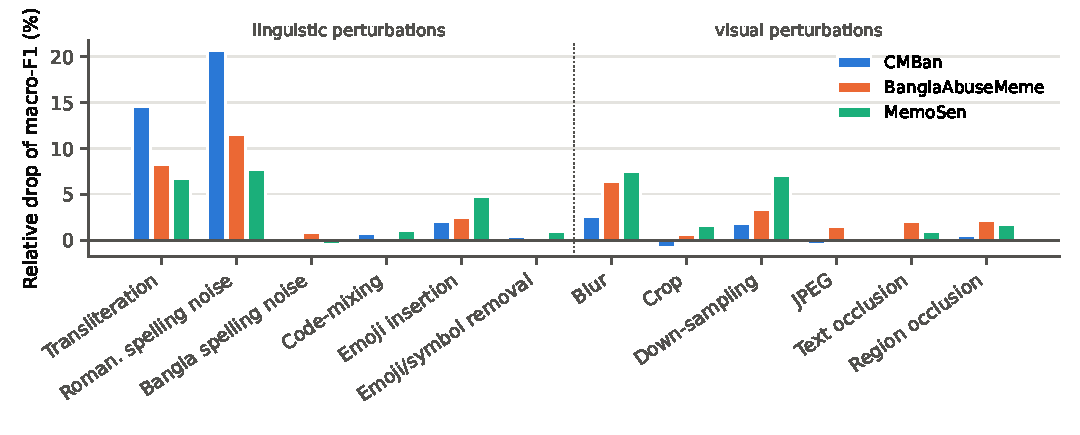
\includegraphics[width=\textwidth]{figures/cross_robustness.pdf}
  \caption{Relative Robustness Drop of the XLM-R + CLIP-B/32 fusion heads (mean over five heads, all tasks and three
  severities) for each perturbation family and dataset.}
  \label{fig:cross_rob}
\end{figure*}

\begin{table*}[t]
\centering
\small
\caption{Relative Robustness Drop (\%) across datasets, averaged over tasks and severities, for the matching unimodal heads (uni.) and the five XLM-R + CLIP-B/32 fusion heads (fus.; flip rate \% in parentheses). The top six rows are linguistic, the bottom six visual perturbations.}
\label{tab:cross_rob}
\begin{adjustbox}{max width=\textwidth}
\begin{tabular}{lcccccc}
\toprule
Perturbation & CMBan uni. & CMBan fus. & BAM uni. & BAM fus. & MemoSen uni. & MemoSen fus. \\
\midrule
Transliteration & 12.9 & 14.5 (37) & 18.4 & 8.2 (22) & 17.3 & 6.7 (21) \\
Roman. spelling noise & 17.9 & 20.7 (45) & 26.5 & 11.5 (28) & 21.8 & 7.7 (26) \\
Bangla spelling noise & 0.6 & 0.3 (7) & 1.7 & 0.8 (6) & 0.3 & -0.5 (8) \\
Code-mixing & -1.5 & 0.7 (8) & 0.7 & 0.3 (4) & 3.0 & 1.1 (8) \\
Emoji insertion & 2.3 & 2.0 (12) & 4.8 & 2.5 (11) & 11.7 & 4.8 (14) \\
Emoji/symbol removal & 1.0 & 0.4 (3) & 0.2 & 0.1 (1) & 3.5 & 0.9 (3) \\
Blur & 2.8 & 2.6 (23) & 16.6 & 6.3 (20) & 14.9 & 7.4 (27) \\
Crop & -1.9 & -0.7 (12) & 0.9 & 0.6 (10) & 3.3 & 1.6 (13) \\
Down-sampling & 2.2 & 1.9 (18) & 8.3 & 3.3 (15) & 13.4 & 7.1 (25) \\
JPEG & -0.0 & -0.5 (6) & 3.2 & 1.5 (8) & 0.8 & -0.1 (7) \\
Text occlusion & -0.3 & 0.3 (14) & 4.4 & 2.0 (11) & 4.0 & 1.0 (17) \\
Region occlusion & 1.4 & 0.5 (10) & 3.8 & 2.1 (11) & 4.5 & 1.6 (12) \\
\bottomrule
\end{tabular}
\end{adjustbox}
\end{table*}


Figure~\ref{fig:cross_rob} and Table~\ref{tab:cross_rob} summarise the Robustness Drop.
Figure~\ref{fig:sev_cmban} shows the CMBan severity curves.

\paragraph{Romanisation is the most damaging perturbation.} On every dataset, Romanised spelling noise is the
single most harmful perturbation for the fusion models. It costs 20.7\% (CMBan), 11.5\% (BAM) and 7.7\% (MemoSen) of
relative macro-F1 and changes 26--45\% of predictions. Transliteration without added noise costs 6.7--14.5\%. For the text-only heads, Romanised spelling noise costs
more still, at 17.9--26.5\%. By contrast, spelling noise in native Bangla script costs at most
1.7\%, and code-mixing at most 3\%. The damage is therefore caused by the \emph{change of script}, not by spelling
variation as such. A Romanised meme is tokenised by XLM-R into a different, and for Banglish poorly trained, part
of its vocabulary, so its embedding moves far from the Bangla-script training distribution.

\paragraph{Fusion mitigates text fragility only with enough data.} With sufficient training data, fusion halves the
damage of Romanisation relative to the text-only heads (BAM: 11.5 vs.\ 26.5\%; MemoSen: 7.7 vs.\ 21.8\%), because the
image branch keeps part of the decision intact. On CMBan the opposite happens. The fusion heads lose \emph{more}
than the text-only heads (20.7 vs.\ 17.9\%), and the Concat-MLP curve tracks the Text-MLP curve almost exactly
(Figure~\ref{fig:sev_cmban}). With 133 training memes, the fusion heads cannot learn to discount an unreliable
text input. Section~\ref{sec:results:xai} shows that, on all datasets, the perturbed text \emph{gains}
attribution share instead of losing it.

\paragraph{Visual robustness depends on how much the model uses the image.} Visual perturbations are almost harmless
on CMBan (at most 2.6\%), but on the larger datasets blur and down-sampling cost the image-only heads 8--17\% and
the fusion heads 3--7\%. On MemoSen, blur (7.4\%) is nearly as harmful as Romanisation (7.7\%). The difference
mirrors the benchmark: on the larger datasets the image models are more accurate and thus have more to lose.
Text-region occlusion, which removes up to all OCR regions from the image, costs only 0.3--2.0\% for fusion, and
JPEG compression and cropping cost the fusion heads at most 1.6\%.

\paragraph{Aggregate F1 hides instability.} Visual perturbations flip many predictions even when macro-F1 barely
moves. On CMBan, blur changes 23\% of fusion predictions at a 2.6\% F1 cost, because correct predictions that break
are offset by wrong predictions that become correct. Under severity-3 blur, 28\% of the memes that the fusion model
classifies correctly on Motivational become wrong. We therefore recommend reporting flip rates alongside Robustness
Drop.

\paragraph{Language groups.} Table~\ref{tab:cross_lang} breaks flip rates down by the script of the meme text.
\begin{itemize}
  \item Bangla-script memes flip most often under Romanisation (23--43\% for transliteration), because the
  perturbation rewrites all of their text.
  \item Code-mixed memes flip less (18--28\%), since part of their text is already in Latin script.
  \item Latin-script memes are, as a sanity check, almost unaffected by transliteration ($\leq$2.5\%). They still
  flip in 9--10\% of cases under spelling noise, which also affects English words.
\end{itemize}
Visual flip rates are similar across groups.

\begin{table}[t]
\centering
\small
\caption{Flip rate (\%) of the fusion heads by script/language group of the meme text.}
\label{tab:cross_lang}
\begin{adjustbox}{max width=\columnwidth}
\begin{tabular}{lcccccc}
\toprule
Dataset & Group & Transliteration & Roman. spelling noise & Code-mixing & Blur & Text occlusion \\
\midrule
CMBan & Bangla & 42.6 & 51.4 & 8.6 & 23.6 & 14.8 \\
CMBan & Code-mixed & 27.8 & 35.2 & 6.0 & 21.5 & 13.9 \\
BAM & Bangla & 23.2 & 29.8 & 4.5 & 20.1 & 10.9 \\
BAM & Code-mixed & 18.5 & 24.5 & 3.5 & 20.4 & 10.7 \\
BAM & Latin-script & 2.5 & 10.4 & 2.4 & 21.2 & 10.4 \\
MemoSen & Bangla & 25.4 & 29.6 & 8.5 & 28.5 & 16.9 \\
MemoSen & Code-mixed & 18.3 & 24.4 & 8.1 & 27.6 & 18.8 \\
MemoSen & Latin-script & 0.6 & 9.2 & 6.3 & 16.3 & 12.5 \\
\bottomrule
\end{tabular}
\end{adjustbox}
\end{table}


\begin{figure*}[t]
  \centering
  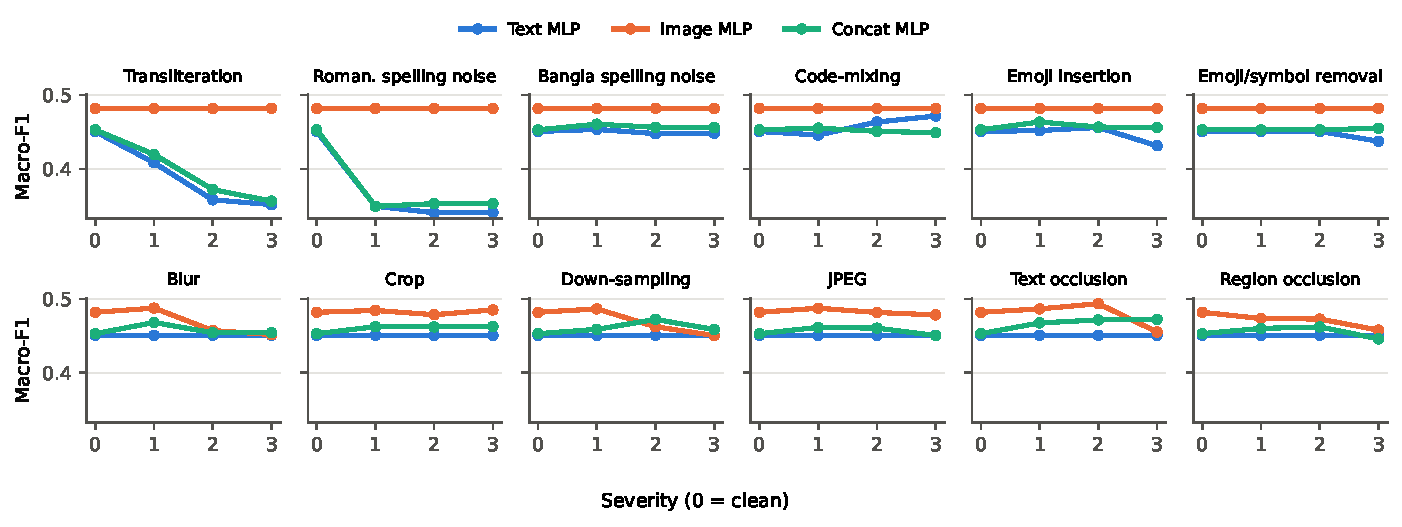
\includegraphics[width=\textwidth]{figures/cmban/severity_curves_coarse.pdf}
  \caption{CMBan: macro-F1 against perturbation severity for the text-only, image-only and Concat-MLP fusion heads
  (XLM-R + CLIP-B/32, coarse labels, mean over tasks).}
  \label{fig:sev_cmban}
\end{figure*}

% =====================================================================================
\subsection{Mitigation: Romanisation Augmentation}
\label{sec:results:aug}

\begin{table*}[t]
\centering
\small
\caption{Train-time Romanisation augmentation (XLM-R + CLIP-B/32). Macro-F1 (\%) on clean test folds and under transliteration and Romanised spelling noise (mean over heads, tasks and severities); relative Robustness Drop (\%) in parentheses. Spelling noise is unseen during training in the \emph{+translit.} setting.}
\label{tab:cross_aug}
\begin{adjustbox}{max width=\textwidth}
\begin{tabular}{lccccccc}
\toprule
Dataset & Augmentation & Text clean & Text translit. & Text noise & Fusion clean & Fusion translit. & Fusion noise \\
\midrule
CMBan & none & 45.5 & 39.7 (13) & 37.5 (18) & 47.2 & 40.6 (15) & 37.8 (21) \\
 & +translit. & 45.6 & 44.1 (3) & 43.2 (5) & 46.5 & 45.3 (2) & 44.0 (5) \\
 & +translit.\,+\,noise & 45.2 & 44.9 (1) & 45.7 (-1) & 46.1 & 46.2 (-1) & 46.0 (-0) \\
BAM & none & 59.2 & 48.2 (18) & 43.4 (26) & 65.0 & 59.8 (8) & 57.7 (12) \\
 & +translit. & 59.5 & 56.0 (6) & 53.7 (10) & 64.9 & 63.5 (2) & 63.1 (3) \\
 & +translit.\,+\,noise & 59.2 & 56.8 (4) & 55.5 (7) & 64.6 & 63.7 (2) & 63.4 (2) \\
MemoSen & none & 46.0 & 38.0 (17) & 36.0 (22) & 53.2 & 49.7 (7) & 49.1 (8) \\
 & +translit. & 45.5 & 43.2 (5) & 40.6 (11) & 53.6 & 52.4 (2) & 51.2 (4) \\
 & +translit.\,+\,noise & 45.2 & 43.7 (3) & 42.5 (6) & 53.5 & 52.7 (2) & 51.9 (3) \\
\bottomrule
\end{tabular}
\end{adjustbox}
\end{table*}


Table~\ref{tab:cross_aug} reports the augmentation experiment of Section~\ref{sec:method:aug}.

\paragraph{Transliteration augmentation removes most of the Romanisation drop.} Adding one transliterated copy of
each training meme reduces the relative drop of the fusion heads under transliteration from 15\% to 2\% on CMBan,
from 8\% to 2\% on BanglaAbuseMeme and from 7\% to 2\% on MemoSen. For the text-only heads, the reduction is from
13--18\% to 3--6\%.

\paragraph{It generalises to an unseen Romanisation style.} Romanised spelling noise is not used for augmentation in
this setting. Even so, the fusion drop under it falls from 21\% to 5\% (CMBan), 12\% to 3\% (BanglaAbuseMeme) and
8\% to 4\% (MemoSen). The heads thus learn to handle Romanised Bangla in general, not just the exact output of our
transliterator. Adding the noise style to training as well (\emph{+translit.\ + noise}) closes the remaining gap,
but only marginally improves on transliteration alone.

\paragraph{Clean accuracy is preserved.} The clean macro-F1 of the fusion heads changes by $-0.7$ (CMBan),
$-0.1$ (BanglaAbuseMeme) and $+0.4$ (MemoSen) points. The other linguistic perturbations are unaffected, apart
from changes of at most 1.3 points. Romanisation augmentation is therefore an almost free remedy for the main
weakness identified in Section~\ref{sec:results:rob}.

% =====================================================================================
\subsection{Explainability}
\label{sec:results:xai}

\begin{table*}[t]
\centering
\small
\caption{Explainability across datasets. Columns 2--8: text share of the Integrated-Gradients attribution of Concat-MLP on clean inputs and at severity 3. CAM ratio: Grad-CAM mass on OCR text boxes divided by their area share ($>1$: over-attention to rendered text). $r$: Pearson correlation of clean vs.\ perturbed CAMs (severity 2).}
\label{tab:cross_xai}
\begin{adjustbox}{max width=\textwidth}
\begin{tabular}{lcccccccccc}
\toprule
Dataset & Clean & Translit. & Roman. noise & Emoji ins. & Blur & Down-samp. & Text occ. & CAM ratio & $r$ blur & $r$ JPEG \\
\midrule
CMBan & 0.59 & 0.73 & 0.72 & 0.62 & 0.50 & 0.51 & 0.51 & 1.13 & 0.30 & 0.92 \\
BanglaAbuseMeme & 0.55 & 0.71 & 0.70 & 0.59 & 0.43 & 0.44 & 0.44 & 0.76 & 0.39 & 0.87 \\
MemoSen & 0.55 & 0.68 & 0.67 & 0.59 & 0.46 & 0.46 & 0.47 & 0.88 & 0.36 & 0.92 \\
\bottomrule
\end{tabular}
\end{adjustbox}
\end{table*}


\paragraph{Modality reliance.} On clean memes, the text embedding receives 55--59\% of the IG attribution of
Concat-MLP (Table~\ref{tab:cross_xai}, Figure~\ref{fig:share_cmban}). The perturbations shift this share in
opposite directions, and the pattern is the same on all three datasets.
\begin{itemize}
  \item \emph{Romanisation increases the text share} to 0.67--0.73. The perturbed text embedding lies far from the
  training mean that serves as the IG baseline, so it dominates the attribution. Instead of discounting an
  unfamiliar input, the head relies on it \emph{more}. This is the mechanism behind the large Romanisation drops.
  \item \emph{Visual degradation decreases the text share} to 0.43--0.51. Blur, down-sampling and text occlusion
  lower it by almost exactly the same amount. All three remove legible text from the image, which suggests that
  much of what the image branch adds to the decision is \emph{read} text that agrees with the text branch.
\end{itemize}

\begin{figure}[t]
  \centering
  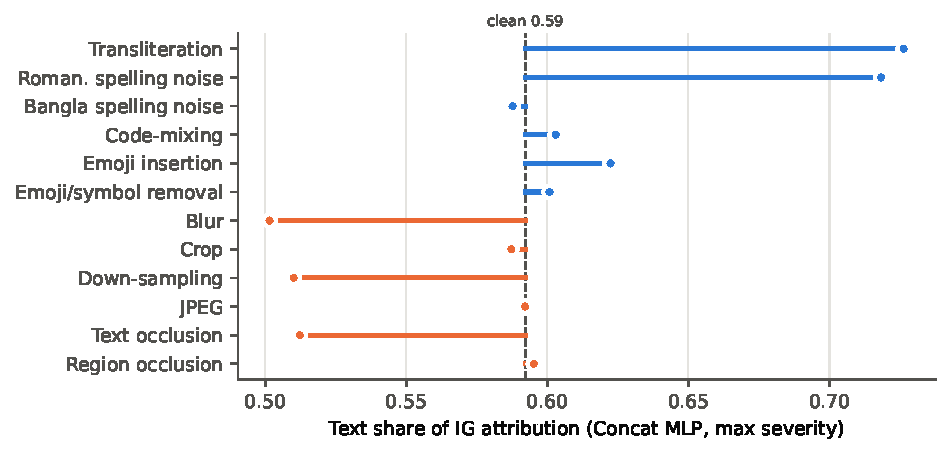
\includegraphics[width=\columnwidth]{figures/cmban/modality_share_shift.pdf}
  \caption{CMBan: shift of the text share of IG attribution (Concat-MLP) from clean inputs (dashed line) to
  severity-3 perturbations. Blue: linguistic, orange: visual. BAM and MemoSen show the same pattern
  (Table~\ref{tab:cross_xai}).}
  \label{fig:share_cmban}
\end{figure}

\paragraph{Visual attention.} The Grad-CAM text-attention ratio of CLIP-B/32 differs between datasets.
\begin{itemize}
  \item On CMBan it is 1.13: CLIP over-attends to the rendered caption, consistent with its known ability to read
  text.
  \item On BAM (0.76) and MemoSen (0.88), the captions receive \emph{less} attention than their area would warrant.
\end{itemize}
CMBan memes are cartoon panels with large speech bubbles, while many BAM and MemoSen memes are photographs with a
short caption band, where faces and scenes compete for attention. The claim that CLIP mainly attends to text
therefore does not generalise beyond cartoon memes.

The stability of the maps is consistent across datasets:
\begin{itemize}
  \item The maps are stable under JPEG compression ($r=0.87$--$0.92$).
  \item They are unstable under blur ($r=0.30$--$0.39$) and down-sampling ($r\approx0.5$--$0.6$), even when the
  prediction is unchanged.
\end{itemize}
Figure~\ref{fig:gradcam_cmban} shows CMBan examples. After text occlusion, the attention moves to the remaining text
and to the cartoon characters. The letterbox padding also attracts attention, which suggests that it should be
masked in future work.

\begin{figure*}[t]
  \centering
  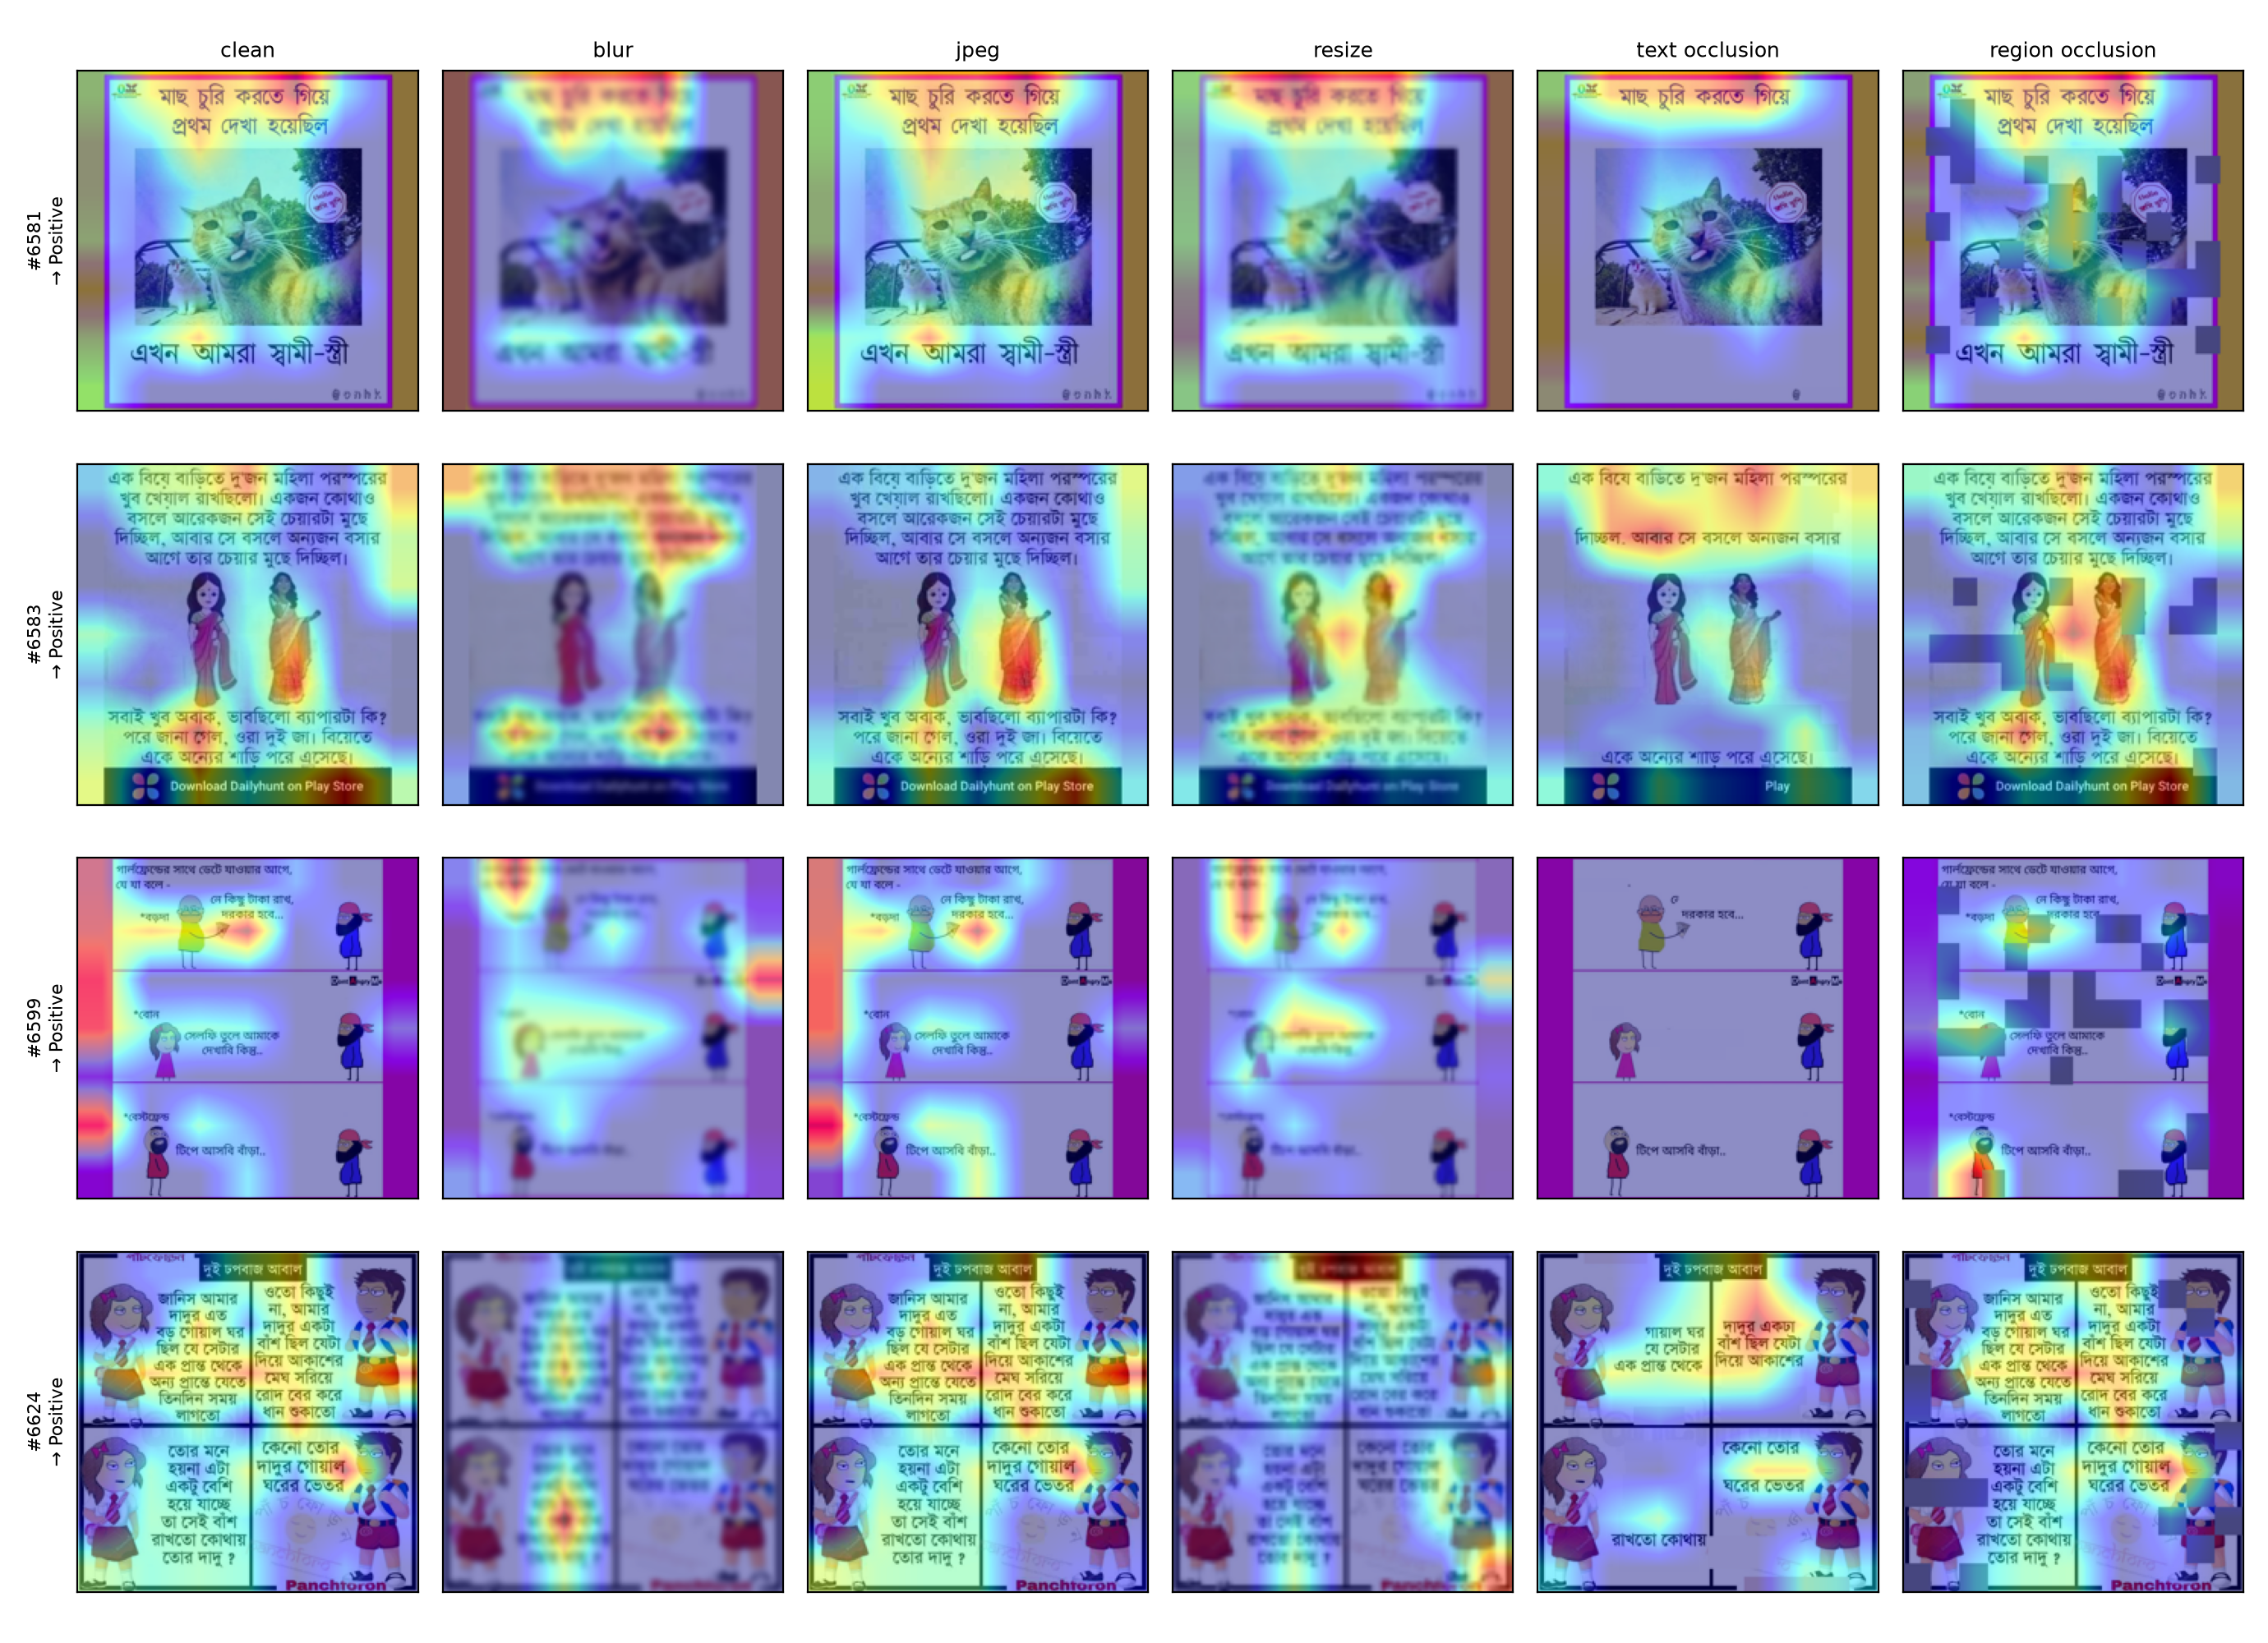
\includegraphics[width=0.85\textwidth]{figures/cmban/gradcam_examples.png}
  \caption{CMBan: Grad-CAM on CLIP ViT-B/32 (sentiment head) for four memes under the spatially aligned visual
  perturbations at severity 2.}
  \label{fig:gradcam_cmban}
\end{figure*}

% =====================================================================================
\subsection{Error Analysis}
\label{sec:results:errors}

\begin{table*}[t]
\centering
\small
\caption{Clean-data error categories of the primary fusion model (\% of memes, averaged over tasks).}
\label{tab:cross_err}
\begin{adjustbox}{max width=\textwidth}
\begin{tabular}{lcccccc}
\toprule
Dataset & Contextual/cultural & Correct & Cross modal & Linguistic & OCR limited & Visual \\
\midrule
CMBan & 17.6 & 55.2 & 3.6 & 8.7 & 6.0 & 8.9 \\
BanglaAbuseMeme & 10.8 & 67.8 & 0.9 & 7.3 & 6.8 & 6.3 \\
MemoSen & 10.4 & 68.5 & 3.2 & 5.7 & 6.3 & 5.8 \\
\bottomrule
\end{tabular}
\end{adjustbox}
\end{table*}

\begin{table}[t]
\centering
\small
\caption{Robustness fragility categories (\% of memes, averaged over tasks; severity $\geq 2$).}
\label{tab:cross_frag}
\begin{adjustbox}{max width=\columnwidth}
\begin{tabular}{lccccc}
\toprule
Dataset & Clean error & Cross modal fragile & Linguistic fragile & Stable & Visual fragile \\
\midrule
CMBan & 43.3 & 20.5 & 18.5 & 11.1 & 6.6 \\
BanglaAbuseMeme & 32.2 & 13.6 & 11.1 & 32.7 & 10.5 \\
MemoSen & 31.2 & 19.3 & 14.7 & 22.2 & 12.7 \\
\bottomrule
\end{tabular}
\end{adjustbox}
\end{table}


\paragraph{Clean errors.} Table~\ref{tab:cross_err} attributes the clean errors of the best learned XLM-R +
CLIP-B/32 fusion head. Late fusion is excluded, because it averages the two unimodal models and cannot, for binary
tasks, fail when both are right.
\begin{itemize}
  \item The largest error category on every dataset is \emph{contextual/cultural}: 18\% of CMBan memes and 10--11\%
  of BAM and MemoSen memes. Here all three models fail although readable text is available.
  \item The category peaks on Sentiment (27\% on CMBan, 18\% on BAM) and on CMBan Sarcasm and Humour (20\%).
  \item The memes in this category typically depend on knowledge outside the meme, such as a film, a public figure
  or a template whose meaning has drifted.
\end{itemize}
Linguistic and visual errors are about equally common (6--9\% each), and OCR-limited errors account for 6--7\%.
\emph{Cross-modal} errors, where both unimodal models are right but fusion is wrong, are rare (1--4\%). The learned
fusion heads seldom destroy information that either modality has, but they also rarely recover memes that both
modalities miss.

\paragraph{Fragility.} Table~\ref{tab:cross_frag} classifies each meme by its behaviour under perturbations of
severity $\geq2$.
\begin{itemize}
  \item Only 11\% (CMBan) to 33\% (BAM) of memes are \emph{stable}: correct on clean data and under every
  perturbation.
  \item Among the memes that are correct on clean data, cross-modal fragility (broken by both a linguistic and a
  visual perturbation) is the most common failure type on all three datasets (13.6--20.5\% of all memes).
  \item On CMBan, linguistic fragility dominates the Offensive task (44\%). Offensive memes are often recognised from
  a few Bangla swear words, which Romanisation disguises.
\end{itemize}

\section{Discussion}
\label{sec:discussion}

\subsection{Revisiting the Expected Findings}
Our project proposal stated six expectations. We revisit them in the light of the results.

\begin{enumerate}
  \item \textbf{Multimodal models outperform unimodal ones on at least some tasks.} \emph{Supported on the larger
  datasets.} Fusion significantly beats the best text model on all five BAM and MemoSen tasks and the best image
  model on two of them. On the 133 labelled CMBan memes the evidence is inconclusive. The gain over the image model
  is small (1.5--2 points), because CLIP already captures much of what the text adds.

  \item \textbf{Humour and sarcasm remain hard.} \emph{Partly supported.} Sentiment, not humour or sarcasm, is the
  hardest task on every dataset. However, CMBan Humour and Sarcasm have the largest share of contextual/cultural
  errors after Sentiment (about 20\%), and BAM Sarcasm is the task where fusion gains least over the image model
  (+0.2 points).

  \item \textbf{Different perturbations affect different models and tasks differently.} \emph{Supported.}
  Linguistic perturbations hurt text and fusion heads, visual ones hurt image and fusion heads, and the effects
  differ by task. Romanisation costs CMBan Offensive 13--18 F1 points and BAM Vulgarity 10--13 points, but leaves
  Sarcasm almost unchanged on both datasets. Tasks signalled by specific words (swear words, slurs) are the most
  vulnerable to a change of script. Sarcasm depends more on the incongruity between image and text, and is the least
  vulnerable.

  \item \textbf{Linguistic perturbations hurt text-heavy memes more; visual corruption hurts where the image is the
  evidence.} \emph{Supported.} Romanisation hurts Bangla-script memes most, whose entire text is rewritten. Visual
  corruptions matter most on the datasets where the image model is strongest (BAM, MemoSen).

  \item \textbf{Explainability reveals modality-specific failure modes.} \emph{Supported, with a surprise.} IG shows
  that Romanised text attracts \emph{more} attribution rather than less. Grad-CAM shows over-attention to rendered
  captions on cartoon memes, but not on photographic memes.

  \item \textbf{The most vulnerable perturbations and dimensions can be identified.} \emph{Supported.} Romanisation
  is the dominant threat on every dataset, followed by blur and down-sampling on the larger datasets. Lexically signalled
  dimensions (offensiveness, vulgarity) and sentiment are the most affected.
\end{enumerate}

\subsection{Why Romanisation Breaks Fusion Models}
Three observations combine into a consistent explanation.
\begin{enumerate}
  \item XLM-R's representation of Romanised Bangla is far from that of Bangla script. Native-script spelling noise
  of similar strength is harmless.
  \item The fusion head has never seen such inputs during training. It treats the out-of-distribution text vector
  as strong evidence, which is reflected in the increased IG text share.
  \item With little training data (CMBan), the head has not learned to rely on the image, so the error propagates
  fully. With more data, the image branch absorbs about half of the damage.
\end{enumerate}
The augmentation experiment (Section~\ref{sec:results:aug}) confirms this account. Showing the head transliterated
copies of its training memes removes most of the drop, including for an unseen Romanisation style. The weakness
therefore lies in the training distribution of the head, not in an inability of the encoder to represent Banglish.

\subsection{Practical Recommendations}
\begin{itemize}
  \item \textbf{Augment with Romanised text.} Transliteration augmentation is cheap, needs no extra labels, and
  removes most of the dominant failure mode at a cost of under one F1 point on clean data.
  \item \textbf{Report flip rates.} Visual perturbations change up to 27\% of predictions with only a few points of
  F1 loss. Aggregate accuracy alone overstates stability.
  \item \textbf{Do not discard character features.} Character $n$-gram models beat frozen sentence encoders on
  meme text. Combining both, or fine-tuning the text encoder, is a promising direction.
  \item \textbf{Prefer a stronger image encoder when affordable.} CLIP ViT-L/14 gives the largest single accuracy
  gain (2.7--2.8 points). The image branch is also what cushions text corruption.
\end{itemize}

\subsection{CMBan in Context}
CMBan's cartoon memes differ from the photographic memes of BAM and MemoSen in three ways:
\begin{itemize}
  \item Their text is longer (24.8 vs.\ about 15 words).
  \item CLIP attends more to their captions.
  \item Their errors are more often contextual or cultural (18\% vs.\ 10--11\%).
\end{itemize}
These differences support CMBan's motivation as a distinct resource: cartoon memes rely heavily on the written
dialogue and on shared cultural knowledge of recurring templates. They also mean that conclusions drawn on
photographic Bangla memes do not automatically transfer to cartoon memes. The full CMBan label release would allow
these differences to be tested with adequate statistical power.

\section{Conclusion}
\label{sec:conclusion}

We presented ToonSense, a robustness study of multimodal classifiers for Bangla--English memes built on frozen
multilingual text encoders and CLIP. Across CMBan cartoon memes and two larger Bangla meme datasets, we benchmarked
six text encoders, four image encoders and five fusion heads, and subjected the primary XLM-R + CLIP-B/32 models to
twelve linguistic and visual perturbations at three severities.

Four conclusions stand out.
\begin{enumerate}
  \item \textbf{Clean accuracy.} The image modality carries most of the signal, and frozen text encoders are
  outperformed even by character $n$-grams. Fusion adds a small but significant gain once a few thousand training
  memes are available.

  \item \textbf{Romanisation is the main threat.} Writing the same meme in Romanised Bangla is the most damaging
  perturbation on every dataset, costing the fusion models 8--21\% of relative macro-F1. Native-script spelling
  noise and code-mixing are nearly harmless. Fusion halves the damage only when enough training data is
  available, and the perturbed text attracts \emph{more} attribution rather than less.

  \item \textbf{A simple remedy.} Adding transliterated copies of the training memes, with no new labels, reduces the Romanisation drop of
  the fusion models from 7--15\% to 2\% for transliteration and from 8--21\% to 3--5\% for an unseen
  Romanised spelling style, while changing clean macro-F1 by less than one point.

  \item \textbf{Stability is not accuracy.} Visual perturbations flip up to 27\% of predictions with little change
  in macro-F1. Robustness evaluations should therefore report flip rates. CLIP's attention to rendered text is a
  property of cartoon memes rather than of memes in general.
\end{enumerate}

Future work should evaluate fine-tuned and generative vision--language models with the same protocol, collect
naturally Romanised versions of existing memes, verify the contextual/cultural error candidates with native
speakers, and repeat the CMBan analyses once its full label set is released.

\section*{Limitations}
\label{sec:limitations}

\begin{itemize}
  \item \textbf{Size of the released CMBan labels.} Only 133 of the 2{,}641 CMBan memes have public labels. On CMBan,
  most differences between models fall within the bootstrap confidence intervals, so CMBan results should be read
  as indicative. We mitigate this with repeated cross-validation, bootstrap intervals and label-free flip rates,
  and by replicating every analysis on BanglaAbuseMeme and MemoSen ($\sim$4k memes each). Two CMBan observations,
  fusion amplifying text fragility and CLIP over-attending to captions, did not replicate on the larger datasets.

  \item \textbf{OCR as the text source.} For CMBan and BanglaAbuseMeme the text modality is produced by EasyOCR
  (mean confidence $0.58$ on CMBan). Part of the text-encoder weakness may therefore reflect OCR errors rather than
  the encoder. MemoSen, which ships human-written captions, partly controls for this.

  \item \textbf{Perturbation coverage.}
  \begin{itemize}
    \item Our code-mixing perturbation is lexicon-based ($\sim$200 words) and changes at most about 19\% of tokens.
    \item OCR output never contains emojis, so emoji \emph{removal} reduces to symbol removal.
    \item The transliterator follows one colloquial convention, whereas real Banglish spelling varies more widely;
    the spelling-noise family approximates this variation.
  \end{itemize}

  \item \textbf{Augmentation and test perturbations share a generator.} The transliteration used for augmentation is
  produced by the same transliterator as the transliteration test perturbation, which favours the augmented models.
  The results under Romanised spelling noise, which is not used for augmentation in the main setting, are the more
  conservative estimate. Gains on naturally written Banglish remain to be confirmed.

  \item \textbf{Decoupled perturbations.} In the main setting each perturbation changes one modality. In real
  circulation, a degraded image also degrades the OCR text. The coupled setting is implemented but was not run at
  full scale.

  \item \textbf{Frozen encoders and selection.} All encoders are frozen, as the proposal specifies. Fine-tuned
  models may behave differently. Robustness and explainability analyses were run for the primary encoder pair only.
  The ``best'' configurations in the fusion-vs-unimodal tests are selected on the same data, which slightly favours
  the selected models.

  \item \textbf{Cultural interpretation.} The \emph{contextual/cultural} error category is detected automatically
  and contains candidates only. Confirming cultural dependence requires native-speaker annotation, which is left
  for future work.
\end{itemize}

\section*{Ethics Statement}
All datasets are publicly released for research:
\begin{itemize}
  \item CMBan under the MIT licence.
  \item BanglaAbuseMeme under CC-BY-4.0.
  \item MemoSen by its authors for research use.
\end{itemize}
Some memes contain offensive, vulgar or abusive content. We use them only to measure model behaviour and do not
redistribute the datasets; the only images reproduced are four non-offensive CMBan examples in the Grad-CAM figure,
shown for illustration. Robustness findings could in principle inform evasion of moderation systems. We report
aggregate vulnerabilities, which are already apparent from everyday social-media writing, rather than methods for
crafting adversarial memes.

\appendices
\section{Per-Dataset Detail Tables}
\label{app:tables}

This appendix lists the full per-dataset tables generated by \texttt{scripts/07\_report.py}. CMBan is reported at
the coarse label level (the fine-level benchmark is included for completeness), and BanglaAbuseMeme and MemoSen at
their released label level.

\subsection{CMBan}
\begin{table*}[t]
\centering
\small
\caption{CMBan: Clean-data benchmark (coarse labels): macro-F1 (\%), mean $\pm$ std over 3 seeds of 5-fold stratified CV.}
\label{tab:bench_coarse_cmban}
\begin{adjustbox}{max width=\textwidth}
\begin{tabular}{lccccccc}
\toprule
Family & Model & Humour & Sarcasm & Offensive & Motivational & Sentiment & Avg. \\
\midrule
Baseline & Majority & 36.4\,$\pm$\,0.0 & 36.4\,$\pm$\,0.0 & 42.7\,$\pm$\,0.0 & 38.4\,$\pm$\,0.0 & 21.0\,$\pm$\,0.0 & 35.0 \\
Baseline & Char TF-IDF LR & 50.7\,$\pm$\,4.5 & 52.7\,$\pm$\,7.6 & 49.6\,$\pm$\,3.2 & 44.6\,$\pm$\,2.1 & 33.5\,$\pm$\,1.8 & 46.2 \\
Text & xlmr-base / Text LR & 45.9\,$\pm$\,1.9 & 48.8\,$\pm$\,4.2 & 49.7\,$\pm$\,4.4 & 46.4\,$\pm$\,2.9 & 38.9\,$\pm$\,3.6 & 45.9 \\
Text & xlmr-large / Text MLP & 49.8\,$\pm$\,3.2 & 51.8\,$\pm$\,2.7 & 47.3\,$\pm$\,0.5 & 48.7\,$\pm$\,2.8 & 32.5\,$\pm$\,5.1 & 46.0 \\
Text & mbert / Text MLP & 47.9\,$\pm$\,3.6 & 48.3\,$\pm$\,6.3 & 43.3\,$\pm$\,4.2 & 51.6\,$\pm$\,2.6 & 33.1\,$\pm$\,4.1 & 44.8 \\
Text & banglabert / Text LR & 51.3\,$\pm$\,4.1 & 49.6\,$\pm$\,5.0 & 50.7\,$\pm$\,7.5 & 50.5\,$\pm$\,2.7 & 31.6\,$\pm$\,5.0 & 46.7 \\
Text & labse / Text MLP & 51.8\,$\pm$\,2.5 & 48.7\,$\pm$\,7.5 & 47.1\,$\pm$\,1.8 & 44.7\,$\pm$\,5.0 & 31.3\,$\pm$\,4.5 & 44.7 \\
Text & me5-base / Text LR & 47.1\,$\pm$\,3.0 & 45.3\,$\pm$\,4.6 & 55.2\,$\pm$\,4.8 & 52.3\,$\pm$\,4.7 & 34.5\,$\pm$\,0.9 & 46.9 \\
Image & clip-b32 / Image MLP & 54.5\,$\pm$\,0.7 & 51.5\,$\pm$\,4.3 & 50.7\,$\pm$\,7.0 & 50.1\,$\pm$\,4.4 & 34.1\,$\pm$\,4.1 & 48.2 \\
Image & clip-b16 / Image LR & 54.8\,$\pm$\,3.0 & 53.7\,$\pm$\,1.4 & 57.0\,$\pm$\,4.8 & 51.4\,$\pm$\,6.7 & 31.8\,$\pm$\,4.8 & 49.7 \\
Image & clip-l14 / Image LR & 56.0\,$\pm$\,3.1 & 55.6\,$\pm$\,1.5 & 53.9\,$\pm$\,2.7 & 59.2\,$\pm$\,1.9 & 30.1\,$\pm$\,3.4 & 51.0 \\
Image & dinov2-base / Image LR & 50.0\,$\pm$\,4.4 & 54.4\,$\pm$\,2.9 & 51.1\,$\pm$\,1.5 & 50.1\,$\pm$\,5.8 & 36.2\,$\pm$\,5.8 & 48.4 \\
Fusion & xlmr-base + clip-b32 / Concat LR & 53.4\,$\pm$\,0.6 & 48.7\,$\pm$\,1.5 & 52.0\,$\pm$\,1.7 & 51.2\,$\pm$\,6.2 & 36.8\,$\pm$\,4.3 & 48.4 \\
Fusion & xlmr-base + clip-b32 / Concat MLP & 47.6\,$\pm$\,3.7 & 49.1\,$\pm$\,1.6 & 45.3\,$\pm$\,5.9 & 49.1\,$\pm$\,0.9 & 35.2\,$\pm$\,0.5 & 45.3 \\
Fusion & xlmr-base + clip-b32 / Late fusion & 51.0\,$\pm$\,5.8 & 52.0\,$\pm$\,0.8 & 52.7\,$\pm$\,6.7 & 50.5\,$\pm$\,8.0 & 34.2\,$\pm$\,3.8 & 48.1 \\
Fusion & xlmr-base + clip-b32 / GMU & 49.6\,$\pm$\,2.1 & 53.9\,$\pm$\,5.3 & 48.9\,$\pm$\,1.9 & 47.5\,$\pm$\,4.5 & 36.5\,$\pm$\,5.6 & 47.3 \\
Fusion & xlmr-base + clip-b32 / Bilinear & 47.5\,$\pm$\,5.6 & 51.8\,$\pm$\,0.7 & 49.2\,$\pm$\,1.3 & 50.2\,$\pm$\,2.3 & 35.5\,$\pm$\,1.6 & 46.9 \\
Fusion & labse + clip-l14 / Concat MLP & 56.0\,$\pm$\,2.7 & 56.8\,$\pm$\,3.5 & 51.6\,$\pm$\,3.0 & 52.0\,$\pm$\,5.6 & 34.0\,$\pm$\,1.4 & 50.1 \\
\bottomrule
\end{tabular}
\end{adjustbox}
\end{table*}

\begin{table*}[t]
\centering
\small
\caption{CMBan: Accuracy, macro precision/recall/F1 of the primary XLM-R + CLIP configuration (coarse).}
\label{tab:primary_coarse_cmban}
\begin{adjustbox}{max width=\textwidth}
\begin{tabular}{lcccccc}
\toprule
Task & Model & Acc & P & R & Macro-F1 & 95\% CI \\
\midrule
Humour & xlmr-base / Text LR & 46.9\,$\pm$\,1.9 & 45.9\,$\pm$\,1.9 & 45.9\,$\pm$\,1.9 & 45.9\,$\pm$\,1.9 & [37.4, 54.6] \\
Humour & xlmr-base / Text MLP & 48.4\,$\pm$\,6.8 & 46.9\,$\pm$\,5.7 & 46.8\,$\pm$\,5.6 & 46.5\,$\pm$\,5.2 & [36.7, 53.6] \\
Humour & clip-b32 / Image LR & 57.6\,$\pm$\,2.4 & 57.1\,$\pm$\,2.4 & 57.2\,$\pm$\,2.4 & 57.1\,$\pm$\,2.4 & [49.5, 65.9] \\
Humour & clip-b32 / Image MLP & 55.6\,$\pm$\,0.8 & 54.6\,$\pm$\,0.6 & 54.5\,$\pm$\,0.6 & 54.5\,$\pm$\,0.7 & [44.2, 61.3] \\
Humour & xlmr-base + clip-b32 / Concat LR & 54.4\,$\pm$\,0.4 & 53.4\,$\pm$\,0.5 & 53.4\,$\pm$\,0.6 & 53.4\,$\pm$\,0.6 & [43.3, 59.9] \\
Humour & xlmr-base + clip-b32 / Concat MLP & 48.6\,$\pm$\,3.6 & 47.7\,$\pm$\,3.7 & 47.7\,$\pm$\,3.7 & 47.6\,$\pm$\,3.7 & [41.4, 59.4] \\
Humour & xlmr-base + clip-b32 / Late fusion & 52.4\,$\pm$\,6.4 & 51.4\,$\pm$\,6.1 & 51.2\,$\pm$\,6.0 & 51.0\,$\pm$\,5.8 & [41.7, 59.5] \\
Humour & xlmr-base + clip-b32 / GMU & 50.1\,$\pm$\,2.2 & 49.6\,$\pm$\,2.0 & 49.6\,$\pm$\,2.0 & 49.6\,$\pm$\,2.1 & [40.9, 57.7] \\
Humour & xlmr-base + clip-b32 / Bilinear & 49.1\,$\pm$\,6.8 & 48.4\,$\pm$\,5.0 & 48.5\,$\pm$\,4.6 & 47.5\,$\pm$\,5.6 & [46.0, 63.3] \\
Sarcasm & xlmr-base / Text LR & 49.9\,$\pm$\,4.3 & 48.9\,$\pm$\,4.2 & 48.8\,$\pm$\,4.2 & 48.8\,$\pm$\,4.2 & [38.0, 54.6] \\
Sarcasm & xlmr-base / Text MLP & 51.4\,$\pm$\,5.7 & 51.6\,$\pm$\,5.4 & 51.6\,$\pm$\,5.5 & 51.2\,$\pm$\,5.6 & [41.1, 57.9] \\
Sarcasm & clip-b32 / Image LR & 47.1\,$\pm$\,4.1 & 45.8\,$\pm$\,3.8 & 45.8\,$\pm$\,3.9 & 45.7\,$\pm$\,3.8 & [36.0, 52.0] \\
Sarcasm & clip-b32 / Image MLP & 51.9\,$\pm$\,3.9 & 51.7\,$\pm$\,4.5 & 51.8\,$\pm$\,4.6 & 51.5\,$\pm$\,4.3 & [41.7, 58.3] \\
Sarcasm & xlmr-base + clip-b32 / Concat LR & 49.9\,$\pm$\,1.6 & 48.7\,$\pm$\,1.5 & 48.7\,$\pm$\,1.5 & 48.7\,$\pm$\,1.5 & [39.2, 55.5] \\
Sarcasm & xlmr-base + clip-b32 / Concat MLP & 49.6\,$\pm$\,1.5 & 49.2\,$\pm$\,1.7 & 49.2\,$\pm$\,1.7 & 49.1\,$\pm$\,1.6 & [42.8, 59.7] \\
Sarcasm & xlmr-base + clip-b32 / Late fusion & 52.6\,$\pm$\,0.8 & 52.0\,$\pm$\,0.8 & 52.0\,$\pm$\,0.8 & 52.0\,$\pm$\,0.8 & [44.3, 62.1] \\
Sarcasm & xlmr-base + clip-b32 / GMU & 54.1\,$\pm$\,5.2 & 54.3\,$\pm$\,5.4 & 54.4\,$\pm$\,5.5 & 53.9\,$\pm$\,5.3 & [46.7, 63.9] \\
Sarcasm & xlmr-base + clip-b32 / Bilinear & 52.4\,$\pm$\,0.9 & 52.0\,$\pm$\,0.8 & 52.0\,$\pm$\,0.8 & 51.8\,$\pm$\,0.7 & [46.0, 62.8] \\
Offensive & xlmr-base / Text LR & 63.9\,$\pm$\,2.0 & 49.7\,$\pm$\,4.7 & 50.0\,$\pm$\,3.9 & 49.7\,$\pm$\,4.4 & [43.0, 60.4] \\
Offensive & xlmr-base / Text MLP & 52.6\,$\pm$\,4.2 & 48.8\,$\pm$\,4.8 & 48.5\,$\pm$\,6.2 & 47.1\,$\pm$\,5.0 & [42.3, 58.6] \\
Offensive & clip-b32 / Image LR & 64.7\,$\pm$\,2.7 & 52.4\,$\pm$\,4.6 & 52.4\,$\pm$\,4.3 & 52.4\,$\pm$\,4.5 & [44.0, 61.8] \\
Offensive & clip-b32 / Image MLP & 55.6\,$\pm$\,8.0 & 52.3\,$\pm$\,5.7 & 52.8\,$\pm$\,7.0 & 50.7\,$\pm$\,7.0 & [45.3, 63.1] \\
Offensive & xlmr-base + clip-b32 / Concat LR & 68.4\,$\pm$\,1.5 & 53.4\,$\pm$\,2.1 & 52.4\,$\pm$\,1.5 & 52.0\,$\pm$\,1.7 & [42.2, 58.8] \\
Offensive & xlmr-base + clip-b32 / Concat MLP & 48.9\,$\pm$\,5.3 & 48.4\,$\pm$\,5.7 & 48.0\,$\pm$\,7.4 & 45.3\,$\pm$\,5.9 & [40.2, 57.0] \\
Offensive & xlmr-base + clip-b32 / Late fusion & 57.9\,$\pm$\,6.7 & 53.7\,$\pm$\,5.8 & 54.7\,$\pm$\,7.2 & 52.7\,$\pm$\,6.7 & [47.1, 64.1] \\
Offensive & xlmr-base + clip-b32 / GMU & 52.9\,$\pm$\,1.6 & 51.2\,$\pm$\,2.1 & 51.6\,$\pm$\,2.7 & 48.9\,$\pm$\,1.9 & [40.8, 57.7] \\
Offensive & xlmr-base + clip-b32 / Bilinear & 56.4\,$\pm$\,4.6 & 50.3\,$\pm$\,0.3 & 50.4\,$\pm$\,0.4 & 49.2\,$\pm$\,1.3 & [43.1, 61.2] \\
Motivational & xlmr-base / Text LR & 48.9\,$\pm$\,2.6 & 46.5\,$\pm$\,3.0 & 46.4\,$\pm$\,3.1 & 46.4\,$\pm$\,2.9 & [41.0, 57.4] \\
Motivational & xlmr-base / Text MLP & 50.1\,$\pm$\,4.1 & 51.4\,$\pm$\,4.0 & 51.4\,$\pm$\,4.3 & 49.8\,$\pm$\,4.1 & [45.1, 62.5] \\
Motivational & clip-b32 / Image LR & 55.9\,$\pm$\,4.3 & 52.1\,$\pm$\,4.3 & 51.9\,$\pm$\,4.0 & 51.9\,$\pm$\,4.0 & [46.8, 64.1] \\
Motivational & clip-b32 / Image MLP & 52.4\,$\pm$\,4.1 & 50.2\,$\pm$\,4.3 & 50.2\,$\pm$\,4.5 & 50.1\,$\pm$\,4.4 & [41.0, 58.6] \\
Motivational & xlmr-base + clip-b32 / Concat LR & 54.9\,$\pm$\,5.3 & 51.2\,$\pm$\,6.3 & 51.3\,$\pm$\,6.0 & 51.2\,$\pm$\,6.2 & [42.6, 59.9] \\
Motivational & xlmr-base + clip-b32 / Concat MLP & 49.4\,$\pm$\,0.9 & 50.8\,$\pm$\,0.9 & 50.8\,$\pm$\,0.9 & 49.1\,$\pm$\,0.9 & [42.3, 58.6] \\
Motivational & xlmr-base + clip-b32 / Late fusion & 51.4\,$\pm$\,8.3 & 51.1\,$\pm$\,7.6 & 51.1\,$\pm$\,8.0 & 50.5\,$\pm$\,8.0 & [39.8, 57.5] \\
Motivational & xlmr-base + clip-b32 / GMU & 47.9\,$\pm$\,4.6 & 48.8\,$\pm$\,4.4 & 48.7\,$\pm$\,4.6 & 47.5\,$\pm$\,4.5 & [35.8, 52.6] \\
Motivational & xlmr-base + clip-b32 / Bilinear & 51.6\,$\pm$\,2.8 & 50.6\,$\pm$\,2.1 & 50.6\,$\pm$\,2.1 & 50.2\,$\pm$\,2.3 & [44.8, 61.9] \\
Sentiment & xlmr-base / Text LR & 40.6\,$\pm$\,4.5 & 39.3\,$\pm$\,3.9 & 38.7\,$\pm$\,3.5 & 38.9\,$\pm$\,3.6 & [29.5, 46.5] \\
Sentiment & xlmr-base / Text MLP & 30.8\,$\pm$\,4.0 & 31.8\,$\pm$\,3.8 & 32.7\,$\pm$\,2.5 & 30.7\,$\pm$\,3.8 & [24.2, 40.2] \\
Sentiment & clip-b32 / Image LR & 32.1\,$\pm$\,4.9 & 30.2\,$\pm$\,5.5 & 30.4\,$\pm$\,5.4 & 30.2\,$\pm$\,5.5 & [22.2, 38.4] \\
Sentiment & clip-b32 / Image MLP & 35.1\,$\pm$\,5.1 & 35.2\,$\pm$\,4.3 & 35.7\,$\pm$\,4.0 & 34.1\,$\pm$\,4.1 & [26.6, 42.4] \\
Sentiment & xlmr-base + clip-b32 / Concat LR & 39.3\,$\pm$\,2.8 & 38.4\,$\pm$\,4.1 & 36.4\,$\pm$\,4.0 & 36.8\,$\pm$\,4.3 & [31.4, 48.0] \\
Sentiment & xlmr-base + clip-b32 / Concat MLP & 35.3\,$\pm$\,0.8 & 36.6\,$\pm$\,0.6 & 36.7\,$\pm$\,0.5 & 35.2\,$\pm$\,0.5 & [24.9, 40.1] \\
Sentiment & xlmr-base + clip-b32 / Late fusion & 34.8\,$\pm$\,3.8 & 35.8\,$\pm$\,3.4 & 35.8\,$\pm$\,3.3 & 34.2\,$\pm$\,3.8 & [28.1, 44.1] \\
Sentiment & xlmr-base + clip-b32 / GMU & 36.8\,$\pm$\,6.0 & 38.1\,$\pm$\,5.3 & 38.2\,$\pm$\,5.7 & 36.5\,$\pm$\,5.6 & [23.7, 39.6] \\
Sentiment & xlmr-base + clip-b32 / Bilinear & 36.6\,$\pm$\,0.4 & 36.2\,$\pm$\,2.5 & 36.5\,$\pm$\,2.3 & 35.5\,$\pm$\,1.6 & [27.6, 43.4] \\
\bottomrule
\end{tabular}
\end{adjustbox}
\end{table*}

\begin{table}[t]
\centering
\small
\caption{CMBan: Fusion grid: task-averaged macro-F1 (\%) of the best fusion head for each encoder pair.}
\label{tab:grid_coarse_cmban}
\begin{adjustbox}{max width=\columnwidth}
\begin{tabular}{lcccc}
\toprule
Text \textbackslash{} Image & clip-b16 & clip-b32 & clip-l14 & dinov2-base \\
\midrule
banglabert & 49.2 & 48.0 & 49.3 & 50.3 \\
labse & 48.6 & 48.0 & 50.3 & 50.0 \\
mbert & 47.4 & 46.9 & 49.5 & 50.3 \\
me5-base & 50.0 & 48.3 & 50.3 & 50.0 \\
xlmr-base & 47.9 & 49.6 & 49.1 & 50.1 \\
xlmr-large & 48.3 & 47.9 & 49.5 & 48.5 \\
\bottomrule
\end{tabular}
\end{adjustbox}
\end{table}

\begin{table*}[t]
\centering
\small
\caption{CMBan: Relative Robustness Drop (\%) of macro-F1, averaged over tasks and severities; flip rate (\%) in parentheses (xlmr-base + clip-b32, coarse).}
\label{tab:rob_coarse_cmban}
\begin{adjustbox}{max width=\textwidth}
\begin{tabular}{lccccccccc}
\toprule
Perturbation & Text LR & Text MLP & Image LR & Image MLP & Concat LR & Concat MLP & GMU & Bilinear & Late fusion \\
\midrule
Transliteration & 8.3 (39) & 17.5 (47) & -- & -- & 12.2 (34) & 16.7 (41) & 16.5 (39) & 13.9 (35) & 13.3 (35) \\
Roman. spelling noise & 11.8 (47) & 24.1 (55) & -- & -- & 16.7 (42) & 23.5 (49) & 21.9 (47) & 21.0 (43) & 20.4 (44) \\
Bangla spelling noise & 1.4 (12) & -0.1 (11) & -- & -- & 0.7 (8) & -1.0 (7) & 1.0 (7) & 0.5 (8) & 0.5 (5) \\
Code-mixing & -0.7 (12) & -2.3 (12) & -- & -- & 0.4 (8) & 0.3 (8) & 0.6 (8) & 1.4 (8) & 1.0 (6) \\
Emoji insertion & 4.0 (19) & 0.7 (17) & -- & -- & 5.1 (13) & -1.0 (13) & 2.0 (13) & 0.7 (11) & 3.2 (10) \\
Emoji/symbol removal & 1.2 (5) & 0.8 (5) & -- & -- & 0.7 (4) & -0.2 (3) & 0.0 (3) & 1.0 (3) & 0.7 (3) \\
Blur & -- & -- & 3.1 (36) & 2.6 (37) & 5.0 (22) & -1.7 (20) & 5.3 (21) & 2.4 (23) & 2.0 (26) \\
Crop & -- & -- & -3.5 (20) & -0.3 (19) & -1.8 (11) & -2.0 (11) & -0.0 (12) & -0.7 (13) & 1.0 (12) \\
Down-sampling & -- & -- & 2.0 (28) & 2.4 (30) & 3.6 (17) & -2.6 (17) & 5.0 (17) & 2.3 (18) & 1.0 (21) \\
JPEG & -- & -- & 0.2 (12) & -0.3 (10) & -0.2 (6) & -1.1 (6) & 0.4 (6) & -1.2 (7) & -0.4 (7) \\
Text occlusion & -- & -- & -0.9 (20) & 0.2 (23) & 2.7 (13) & -4.1 (14) & 2.0 (14) & 1.5 (15) & -0.5 (16) \\
Region occlusion & -- & -- & 0.1 (19) & 2.7 (18) & -0.6 (10) & -0.8 (8) & 1.4 (9) & -0.0 (11) & 2.6 (12) \\
\bottomrule
\end{tabular}
\end{adjustbox}
\end{table*}

\begin{table}[t]
\centering
\small
\caption{CMBan: Absolute macro-F1 drop (points) per task for the most robust fusion head (Concat MLP).}
\label{tab:rob_task_coarse_cmban}
\begin{adjustbox}{max width=\columnwidth}
\begin{tabular}{lccccc}
\toprule
Perturbation & Humour & Motivational & Offensive & Sarcasm & Sentiment \\
\midrule
Transliteration & 5.1 & 6.1 & 13.1 & -0.7 & 11.5 \\
Roman. spelling noise & 11.3 & 9.4 & 17.7 & -0.9 & 13.1 \\
Bangla spelling noise & -0.7 & -0.2 & -0.3 & -1.5 & 0.4 \\
Code-mixing & -0.0 & 0.4 & 0.5 & -0.9 & 0.6 \\
Emoji insertion & 0.1 & -2.8 & -1.5 & -0.4 & 1.8 \\
Emoji/symbol removal & -0.1 & 0.4 & -0.7 & 0.2 & -0.2 \\
Blur & 2.1 & -1.3 & -0.6 & -1.8 & -1.4 \\
Crop & 0.0 & -1.1 & -2.0 & -2.3 & 0.6 \\
Down-sampling & 2.2 & -1.1 & -2.2 & -2.3 & -1.8 \\
JPEG & -0.2 & -0.7 & -0.4 & -0.6 & -0.4 \\
Text occlusion & 1.3 & -1.6 & -4.1 & -3.0 & -1.5 \\
Region occlusion & -0.6 & 0.1 & 0.5 & -1.2 & -0.4 \\
\bottomrule
\end{tabular}
\end{adjustbox}
\end{table}

\begin{table}[t]
\centering
\small
\caption{CMBan: Grad-CAM analysis: CAM mass on OCR text regions vs. their area share (ratio $>1$: over-attention to rendered text) and Pearson $r$ between clean and perturbed CAMs.}
\label{tab:gradcam_cmban}
\begin{adjustbox}{max width=\columnwidth}
\begin{tabular}{lcccccccc}
\toprule
Task & CAM on text & Text area & Ratio & $r$ blur & $r$ jpeg & $r$ resize & $r$ text occ. & $r$ region occ. \\
\midrule
Humour & 0.27 & 0.24 & 1.11 & 0.29 & 0.92 & 0.52 & 0.62 & 0.65 \\
Motivational & 0.29 & 0.24 & 1.23 & 0.30 & 0.91 & 0.47 & 0.59 & 0.65 \\
Offensive & 0.24 & 0.24 & 0.98 & 0.31 & 0.93 & 0.52 & 0.65 & 0.67 \\
Sarcasm & 0.26 & 0.24 & 1.10 & 0.28 & 0.92 & 0.49 & 0.60 & 0.64 \\
Sentiment & 0.29 & 0.24 & 1.25 & 0.32 & 0.94 & 0.52 & 0.62 & 0.70 \\
\bottomrule
\end{tabular}
\end{adjustbox}
\end{table}

\begin{table}[t]
\centering
\small
\caption{CMBan: Clean-data error categories of the primary fusion model (\% of memes).}
\label{tab:clean_error_table_cmban}
\begin{adjustbox}{max width=\columnwidth}
\begin{tabular}{lcccccc}
\toprule
Task & Contextual/cultural & Correct & Cross modal & Linguistic & OCR limited & Visual \\
\midrule
Humour & 19.5 & 53.4 & 3.8 & 9.8 & 6.0 & 7.5 \\
Motivational & 12.8 & 55.6 & 4.5 & 9.0 & 3.8 & 14.3 \\
Offensive & 8.3 & 69.2 & 3.0 & 8.3 & 2.3 & 9.0 \\
Sarcasm & 20.3 & 55.6 & 3.0 & 6.8 & 8.3 & 6.0 \\
Sentiment & 27.1 & 42.1 & 3.8 & 9.8 & 9.8 & 7.5 \\
\bottomrule
\end{tabular}
\end{adjustbox}
\end{table}

\begin{table}[t]
\centering
\small
\caption{CMBan: Robustness fragility categories (\% of memes; severity $\geq$ 2).}
\label{tab:fragility_table_cmban}
\begin{adjustbox}{max width=\columnwidth}
\begin{tabular}{lccccc}
\toprule
Task & Clean error & Cross modal fragile & Linguistic fragile & Stable & Visual fragile \\
\midrule
Humour & 43.6 & 25.6 & 11.3 & 9.8 & 9.8 \\
Motivational & 43.6 & 23.3 & 6.0 & 13.5 & 13.5 \\
Offensive & 29.3 & 12.8 & 44.4 & 11.3 & 2.3 \\
Sarcasm & 42.9 & 18.8 & 18.8 & 15.8 & 3.8 \\
Sentiment & 57.1 & 21.8 & 12.0 & 5.3 & 3.8 \\
\bottomrule
\end{tabular}
\end{adjustbox}
\end{table}

\begin{table*}[t]
\centering
\small
\caption{CMBan: Clean-data benchmark (fine labels): macro-F1 (\%), mean $\pm$ std over 3 seeds of 5-fold stratified CV.}
\label{tab:bench_fine_cmban}
\begin{adjustbox}{max width=\textwidth}
\begin{tabular}{lccccccc}
\toprule
Family & Model & Humour & Sarcasm & Offensive & Motivational & Sentiment & Avg. \\
\midrule
Baseline & Majority & 20.5\,$\pm$\,0.0 & 20.0\,$\pm$\,0.0 & 28.4\,$\pm$\,0.0 & 38.4\,$\pm$\,0.0 & 12.6\,$\pm$\,0.0 & 24.0 \\
Baseline & Char TF-IDF LR & 34.3\,$\pm$\,2.3 & 33.3\,$\pm$\,2.3 & 29.3\,$\pm$\,1.7 & 44.6\,$\pm$\,2.1 & 15.1\,$\pm$\,1.3 & 31.3 \\
Text & xlmr-base / Text LR & 29.4\,$\pm$\,3.5 & 26.3\,$\pm$\,1.5 & 32.4\,$\pm$\,4.5 & 46.4\,$\pm$\,2.9 & 18.0\,$\pm$\,1.4 & 30.5 \\
Text & xlmr-large / Text LR & 28.8\,$\pm$\,2.7 & 26.0\,$\pm$\,6.0 & 45.7\,$\pm$\,2.9 & 42.9\,$\pm$\,2.6 & 18.0\,$\pm$\,2.7 & 32.3 \\
Text & mbert / Text LR & 31.8\,$\pm$\,2.9 & 29.4\,$\pm$\,2.8 & 31.0\,$\pm$\,1.9 & 57.0\,$\pm$\,3.0 & 22.7\,$\pm$\,3.3 & 34.4 \\
Text & banglabert / Text LR & 38.8\,$\pm$\,3.3 & 33.3\,$\pm$\,4.2 & 35.5\,$\pm$\,2.1 & 50.5\,$\pm$\,2.7 & 21.7\,$\pm$\,4.1 & 36.0 \\
Text & labse / Text LR & 30.0\,$\pm$\,4.8 & 27.7\,$\pm$\,7.8 & 32.1\,$\pm$\,0.6 & 53.5\,$\pm$\,1.4 & 14.6\,$\pm$\,3.0 & 31.6 \\
Text & me5-base / Text LR & 27.4\,$\pm$\,1.6 & 28.4\,$\pm$\,3.8 & 36.6\,$\pm$\,0.5 & 52.3\,$\pm$\,4.7 & 22.5\,$\pm$\,3.6 & 33.4 \\
Image & clip-b32 / Image LR & 44.2\,$\pm$\,5.1 & 25.4\,$\pm$\,4.3 & 32.1\,$\pm$\,0.5 & 51.9\,$\pm$\,4.0 & 18.8\,$\pm$\,1.1 & 34.5 \\
Image & clip-b16 / Image LR & 38.4\,$\pm$\,2.8 & 35.6\,$\pm$\,3.7 & 35.5\,$\pm$\,3.3 & 51.4\,$\pm$\,6.7 & 24.6\,$\pm$\,1.5 & 37.1 \\
Image & clip-l14 / Image LR & 40.1\,$\pm$\,4.4 & 33.8\,$\pm$\,1.6 & 33.4\,$\pm$\,2.4 & 59.2\,$\pm$\,1.9 & 21.5\,$\pm$\,2.8 & 37.6 \\
Image & dinov2-base / Image LR & 36.9\,$\pm$\,1.6 & 30.3\,$\pm$\,5.6 & 36.9\,$\pm$\,4.3 & 50.1\,$\pm$\,5.8 & 20.8\,$\pm$\,1.3 & 35.0 \\
Fusion & xlmr-base + clip-b32 / Concat LR & 35.9\,$\pm$\,5.1 & 25.9\,$\pm$\,2.3 & 31.8\,$\pm$\,2.3 & 51.2\,$\pm$\,6.2 & 15.9\,$\pm$\,2.9 & 32.1 \\
Fusion & xlmr-base + clip-b32 / Concat MLP & 29.9\,$\pm$\,2.7 & 33.1\,$\pm$\,2.4 & 25.0\,$\pm$\,2.7 & 49.1\,$\pm$\,0.9 & 15.1\,$\pm$\,0.8 & 30.4 \\
Fusion & xlmr-base + clip-b32 / Late fusion & 33.3\,$\pm$\,1.2 & 31.5\,$\pm$\,4.9 & 27.1\,$\pm$\,4.4 & 50.5\,$\pm$\,8.0 & 13.3\,$\pm$\,2.0 & 31.1 \\
Fusion & xlmr-base + clip-b32 / GMU & 32.3\,$\pm$\,4.9 & 32.0\,$\pm$\,2.7 & 28.2\,$\pm$\,1.1 & 47.5\,$\pm$\,4.5 & 19.1\,$\pm$\,3.3 & 31.8 \\
Fusion & xlmr-base + clip-b32 / Bilinear & 34.3\,$\pm$\,0.4 & 30.6\,$\pm$\,4.2 & 31.8\,$\pm$\,1.5 & 50.2\,$\pm$\,2.3 & 17.0\,$\pm$\,2.5 & 32.8 \\
Fusion & mbert + dinov2-base / Concat MLP & 34.1\,$\pm$\,3.1 & 38.1\,$\pm$\,2.2 & 31.0\,$\pm$\,2.2 & 52.8\,$\pm$\,1.9 & 18.6\,$\pm$\,2.5 & 34.9 \\
\bottomrule
\end{tabular}
\end{adjustbox}
\end{table*}


% Tables of the two larger datasets are included when present.
\newcommand{\inputifexists}[1]{\IfFileExists{#1}{\input{#1}}{}}

\subsection{BanglaAbuseMeme}
\inputifexists{tables/banglaabusememe/dataset_stats.tex}
\inputifexists{tables/banglaabusememe/benchmark_fine.tex}
\inputifexists{tables/banglaabusememe/fusion_grid_fine.tex}
\inputifexists{tables/banglaabusememe/robustness_fine.tex}
\inputifexists{tables/banglaabusememe/gradcam.tex}
\inputifexists{tables/banglaabusememe/clean_error_table.tex}

\subsection{MemoSen}
\inputifexists{tables/memosen/dataset_stats.tex}
\inputifexists{tables/memosen/benchmark_fine.tex}
\inputifexists{tables/memosen/fusion_grid_fine.tex}
\inputifexists{tables/memosen/robustness_fine.tex}
\inputifexists{tables/memosen/gradcam.tex}
\inputifexists{tables/memosen/clean_error_table.tex}



\section*{Acknowledgment}
We thank our instructor, Antu Chowdhury (Lecturer, SOSET, East Delta University), for guidance throughout this
project.

\bibliographystyle{IEEEtran}
\bibliography{references}
\end{document}
